\documentclass[12pt]{extarticle}
\usepackage{geometry}
\geometry{
a4paper,
total={170mm,257mm},
left=20mm,
top=20mm,
headheight=12pt
}


\usepackage{parskip} % Activate to begin paragraphs with an empty line rather than an indent
\setlength{\parindent}{25pt} % This sets the indentation length for each paragraph
\usepackage{graphicx} % Use pdf, png, jpg, or eps§ with pdflatex; use eps in DVI mode
% TeX will automatically convert eps --> pdf in pdflatex
\usepackage[labelfont=bf]{caption}
\usepackage{float}

\usepackage{amssymb,amsmath,amsthm}
\usepackage{commath}
\usepackage[hyphens]{url}
\usepackage[dvipsnames]{xcolor}
\usepackage[unicode=true,colorlinks=true,urlcolor=CadetBlue,citecolor=black,linkcolor=black]{hyperref}
\PassOptionsToPackage{hyphens}{url} % url is loaded by hyperref
\usepackage{authblk}
\usepackage{longtable}
\usepackage{multirow}
\usepackage{booktabs}
\usepackage{lipsum}  
\usepackage[title,page]{appendix}
\usepackage{chngcntr}
%\usepackage{end float}
 \usepackage{subcaption}
 \usepackage{cleveref}

%SetFonts
% newtxtext+newtxmath
\usepackage{newtxtext} %loads helv for ss, txtt for tt
\usepackage{amsmath}
\usepackage[bigdelims]{newtxmath}
\usepackage[T1]{fontenc}
\usepackage{textcomp}
%SetFonts

% less space before sections 
% https://tex.stackexchange.com/a/101126
%\usepackage{titlesec}
%\titlespacing*{\section}{0pt}{0.5\baselineskip}{0\baselineskip}
%\titlespacing*{\subsection}{0pt}{0.5\baselineskip}{0\baselineskip}
    
% Species names
%% Meta-Command for defining new species macros
\usepackage{xspace}

\allowdisplaybreaks

\newcommand{\species}[3]{%
  \newcommand{#1}{\gdef#1{\textit{#3}\xspace}\textit{#2}\xspace}}
  \species{\yeast}{Saccharomyces cerevisiae}{S.~cerevisiae}


% highlight
\newcommand{\hl}[1]{\colorbox{yellow!50}{$\displaystyle#1$}}

% line numbers
\usepackage[mathlines]{lineno}
\renewcommand\linenumberfont{\normalfont\small\sffamily}
\linenumbers
\modulolinenumbers[2]

% widow and orphan
\widowpenalty=10000
\clubpenalty=10000

% Yoav & Lee commands
\newcommand*{\tr}{^\intercal}
\let\vec\mathbf
\newcommand{\matrx}[1]{{\Big[ \stackrel{}{#1}\Big]}}
\newcommand{\diag}[1]{\mbox{diag}\matrx{#1}}
\newcommand{\goesto}{\rightarrow}
\newcommand{\dspfrac}[2]{\frac{\displaystyle #1}{\displaystyle #2} }
\newtheorem{theorem}{Theorem}
\newtheorem{corollary}{Corollary}
\newtheorem{lemma}{Lemma}
\newtheorem{remark}{Remark}
\newtheorem{result}{Result}
\renewcommand\qedsymbol{} % no square at end of proof
\newcommand{\cl}{\mathbf{L}}
\newcommand{\cj}{\mathbf{J}}
\newcommand{\ci}{\mathbf{I}}
\newcommand{\E}{\mathbf{E}}
\DeclareMathOperator{\sign}{sign}
\renewcommand{\d}[1]{\ensuremath{\operatorname{d}\!{#1}}}

% Remus commands
\newcommand{\x}{{\bf x}}
\renewcommand{\d}{{\rm d}}
\newcommand{\e}{e}
\newcommand{\erfc}{{\rm erfc}}
\newcommand{\ii}{{\rm i}}

\newcommand{\tmi}{\tau_0\wedge\tau}
\newcommand{\tma}{\tau_0\vee\tau}
\newcommand{\taua}{\tau_{\rm A}}

% Daniel commands

\newcommand{\daniel}[1]{\textcolor{blue}{#1}}
\newcommand{\presc}{p_\text{rescue}}
\newcommand{\psgv}{p_\text{SGV}}
\newcommand{\bigo}[1]{\mathcal{O}\left(#1\right)}

% Change Delta to r
\renewcommand{\Delta}{r}

% Supplementary
% https://support.authorea.com/en-us/article/how-to-create-an-appendix-section-or-supplementary-information-1g25i5a/
\newcommand{\beginsupplement}{%
      	\setcounter{table}{0}
        \renewcommand{\thetable}{S\arabic{table}}%
        \setcounter{figure}{0}
        \renewcommand{\thefigure}{S\arabic{figure}}%
		\setcounter{equation}{0}
        \renewcommand{\theequation}{A\arabic{equation}}%
}

% autoref
\def\equationautorefname{Eq.}

% NatBib
\usepackage[comma,sort]{natbib}

%%%%%%%%%%%%%%%%%%%%%%%%%%%%%%%%%%%%%%%%%%%%%%%%%%%%%%

% Title page
\title{
	Evolutionary rescue by aneuploidy in tumors exposed to anti-cancer drugs 
}
% Authors
\renewcommand\Affilfont{\small}

\author[1]{Remus Stana}
\author[2]{Uri Ben-David}
\author[3]{Daniel B. Weissman}
\author[1,*]{Yoav Ram}
\affil[1]{School of Zoology, Faculty of Life Sciences, Tel Aviv University, Tel Aviv, Israel}
\affil[2]{Department of Human Molecular Genetics and Biochemistry, Faculty of Medicine, Tel Aviv University, Tel Aviv, Israel}
\affil[3]{Department of Physics, Emory University, Atlanta, GA, USA}
\affil[*]{Corresponding author: Yoav Ram (e-mail: yoavram@tauex.tau.ac.il)}
 
%%%%%%%%%%%%%%%%%%%%%%%%%%%%%%%%%%%%%%%%%%
\begin{document}
\maketitle

%%%%%%%%%%%%%%%%%%%%%%%%%%%%%%%%%%%%%%%%%%
\begin{abstract}
Evolutionary rescue occurs when a population, facing a sudden environmental change that would otherwise lead to extinction, adapts through beneficial mutations, allowing it to recover and persist.  % change 32
A prime example of evolutionary rescue is the ability of cancer to survive exposure to treatment. 
One evolutionary mechanism by which a population of cancer cells can adapt to chemotherapy is aneuploidy. 
Aneuploid cancer cells can be more fit in an environment altered by anti-cancer drugs, e.g., because aneuploidy disrupts the pathways usually targeted by the drugs. %change 3 
Indeed, aneuploidy is highly prevalent in tumors, and some anti-cancer drugs fight cancer by increasing chromosomal instability.
Here, we model the impact of aneuploidy on the fate of a population of cancer cells. We use multi-type branching processes to approximate the probability that a tumor survives drug treatment as a function of the initial tumor size, the rates at which aneuploidy and other beneficial mutations occur, and the growth rates of the drug-sensitive and drug-resistant cells. Additionally, we investigate the effect of the pre-existent aneuploid cells on the probability of evolutionary rescue.  Finally, we estimate the tumor's mean recurrence time to revert to its initial size following treatment and evolutionary rescue.
We propose that aneuploidy can play an essential role in the relapse of smaller secondary tumors.
\end{abstract}

Keywords: aneuploidy, evolutionary model, adaptive evolution, cancer, drug resistance, chromosome instability

\newpage
%%%%%%%%%%%%%%%%%%%%%%%%%%%%%%%%%%%%%%
\section*{Introduction}

%%%%%%

\paragraph{Aneuploidy in cancer.}  
Each year, approximately 10 million people die from cancer globally \citep{kocarnik2022cancer}. Understanding the factors that contribute to the failure of interventions is of great importance. %change 30
One suggested factor is aneuploidy, in which cells are characterized by an imbalanced karyotype and alterations in the number of chromosomes \citep{schukken2018cin}. 
Aneuploidy is caused by chromosomal instability and mis-segregation of chromosomes during mitosis. Importantly, changes in the number of chromosomes and chromosome arm copies allow cancer cells to survive under stressful conditions such as drug therapy \citep{lukow2021chromosomal,rutledge2016selective,ippolito2021gene}. %change 4
Indeed, cancer cells are often aneuploid, and aneuploidy is associated with poor patient outcomes \citep{ben2020context,smith2018systematic}. 

 \citet{ippolito2021gene} induced aneuploidy in cancer cell lines by exposing them to reversine, a small-molecule inhibitor of the mitotic kinase Mpsi1, and then to anti-cancer drugs such as vemurafenib. Reversine-treated cells had a higher proliferation rate following drug exposure than sensitive cancer cells, due to selection of specific beneficial karyotypes.
Similarly, \citet{lukow2021chromosomal} induced aneuploidy in cancer cells and observed that such cells have an advantage compared to sensitive cells during drug treatment despite having lower fitness before the onset of treatment.
One proposed mechanism through which aneuploidy can confer resistance to anti-cancer drugs is by extending the length of the cell cycle, which prevents the drugs from damaging DNA and microtubules \citep{replogle2020aneuploidy}. Other mechanisms are the selection for specific karyotypes that lead to reduced drug metabolism \citep{ippolito2021gene} and elevated levels of DNA damage repair due to higher basal levels of DNA damage \citep{zerbib2023human}. %change 34
 
An essential aspect of aneuploidy is that the rate with which cells become aneuploid, that is, the rate of chromosome missegregation, is several orders of magnitude higher than mutation rate \citep{bakker2023predicting}. Consequently, a cell exposed to stress, such as chemotherapeutic drugs, can acquire aneuploidy faster than a mutation.
Futhermore, some proposed anti-cancer drugs elevate the missegregation rate to fight cancer cells~\citep{lee2016effects}, as an extremely high chromosome missegregation rate is incompatible with cell survival and proliferation. % change x1

\paragraph{Evolutionary rescue.} Populations adapted to a specific environment are vulnerable to environmental changes, which might cause the population's extinction. Examples of such environmental changes include climate change, invasive species, and the onset of drug therapies. Adaptation is a race against time as the population size decreases in the new environment~\citep{tanaka2022surviving}. 
\emph{Evolutionary rescue} is the process by which the population acquires an adaptation that increases fitness in the new environment such that extinction is averted.
There are three potential ways for a population to survive environmental change \citep{alexander2014evolutionary,bell2017evolutionary}: % change 45 %change 28
migration to a new habitat similar to the one before the onset of environmental change \citep{harsch2014keeping,cobbold2020should,zhou2022range}; 
adaptation by phenotypic plasticity without genetic modification \citep{carja2019evolutionary,carja2017evolutionary,levien2021non,gunnarsson2020understanding}; 
and adaptation through genetic modifications, e.g., mutation \citep{gomulkiewicz1995does,uecker2014evolutionary,uecker2016role,uecker2011fixation,orr2014population}. 
Here, we focus on the latter. 

There has been extensive theoretical analysis of evolutionary rescue.
\citet{orr2008population,orr2014population} thoroughly investigated the simplest case in which there is a specific single mutation or low-frequency variant that is sufficient to rescue the population. 
\citet{martin2013probability} extended these results to consider the effects of a range of rescue genotypes that can vary in both growth rate and variance in offspring number.
\citet{uecker2016role} modeled a situation in which \textit{two} mutations at different loci (with recombination between them) are necessary for rescue. 
\citet{osmond_genetic_2020} considered a population that must achieve rescue, potentially via multiple mutations, by adapting on a fitness landscape described by Fisher's geometric model,
and found that for some parameter values rescue by two mutational steps is more likely than rescue by a single step.

Resistance to cancer therapy is a natural application of evolutionary rescue theory \citep{alexander2014evolutionary}. 
\citet{iwasa2003evolutionary} used multi-type branching process theory to approximate the probability that a population under strong selective pressure can survive extinction, focusing on the case in which the cancer must get two mutations to be rescued, with the single-mutant still dying rapidly.
\citet{iwasa2004evolutionary} used a similar approach to find simple approximate expressions for the probability that a single lineage would evolve to survive via a wide range of possible mutational pathways.
A very similar set of models describe adaptation to new environments (e.g., a pathogen evolving to cross a species barrier) and fitness valley crossing \citep{antia2003role, weissman2009rate}.
\citet{gunnarsson2020understanding} analyzed a model where a tumor consisting of two populations of cancer cells, one drug-resistant and the other drug-sensitive, can evade extinction by cells switching between the two phenotypes through epigenetic mutations. They found that even when drug-resistant cells are barely viable, the epimutations guarantee evolutionary rescue. 

%Evolutionary rescue may occur when a beneficial mutation appears in a single copy, leading to hard selective sweeps, or when multiple mutations appear independently in different individuals, leading to soft selective sweeps. \citet{wilson2017soft} have shown that evolutionary rescue is significantly enhanced by soft selective sweeps when multiple mutations contribute towards evolutionary rescue. Additionally, \citet{osmond_genetic_2020} have calculated the probability that rescue is soft and the expected number of rescue mutations in different scenarios. Evolutionary rescue that requires two successive mutations (i.e., two steps) has been investigated by \citet{martin2013probability}, who tested their model's predictions with data from yeast and bacteria experiments.  %change 41

Here, we study evolutionary rescue after a sudden environmental change caused by initiating anti-cancer drug treatment. 
We consider a range of effects of aneuploidy, from tolerance to (partial) resistance to the drug \citep{brauner2016distinguishing}; note that we use tolerant to refer to aneuploids which have negative growth rates, which is different from other references in the literature such as \citet{berman2020drug}. %change 47
We estimate the effect of aneuploidy on the tumor's evolutionary rescue probability. 
When aneuploidy provides drug resistance, it can directly rescue the tumor. However, when aneuploidy provides tolerance to the drug, it may act as an evolutionary ``stepping stone'' or ``springboard'' \citep{Yona2015,martin2013probability,osmond_genetic_2020}, delaying extinction, and thereby allowing the tumor more time to acquire a resistance mutation on top of the aneuploid background. 
As mentioned above, evidence suggests that aneuploidy may be a common strategy for tumor adaptation to drug therapy. Still, it is unknown how often aneuploidy provides tolerance and acts as a stepping stone.
We also estimate the mean time until a tumor cell population reaches its pre-treatment size following drug therapy. 
Given that aneuploidy is present in many tumors before the onset of therapy \citep{lukow2021chromosomal,ben2020context}, we also consider the effect of pre-treatment standing genetic variation on the evolutionary dynamics. Additionally, we are interested in the timescale of evolutionary rescue and the impact that aneuploidy has on the time necessary for the tumor to overcome drug therapy. 

We will address these questions essentially by combining known results from the evolutionary rescue literature, and considering the quantities and parameter values that are relevant for cancer.
Because these results are scattered across multiple papers, and because they all follow from simple branching process approximations, we re-derive all results here for our model.
While our focus is on the application of evolutionary rescue theory to the evolution of drug resistance in cancer, our model is a general one, and in the general evolutionary rescue context, this work can be seen as a characterization of the circumstances in which two-step processes contribute to rescue even when single-step rescue mutations are available.
This is similar to part of \citet{osmond_genetic_2020} but focused on a different fitness landscape.


%%%%%%%%%%%%%%%%%%%%%%%%%%%%%%%%%%%%%%%%%%
\section*{Methods}

\paragraph{Evolutionary model.}
We follow the number of cancer cells with one of three different genotypes at time $t$: sensitive, $s_t$; tolerant/resistant aneuploid, $a_t$; and resistant mutant, $m_t$. 
These cells divide and die with rates $\lambda_k$ and $\mu_k$ (for $k=s, a, m$).
The division and death rate difference is $\Delta_k = \lambda_k-\mu_k$.
We assume the population of cells is under a strong stress, such as drug therapy, and therefore $\Delta_s<0$, whereas the mutant is resistant to the stress, $\Delta_m>0$.
We consider a range of possible values for $\Delta_a$, finding three distinct scenarios: in the first, aneuploid cells are partially resistant, $\Delta_m>\Delta_a>0$; in the second, aneuploid cells are tolerant, $0>\Delta_a>\Delta_s$ \citep[see][for the distinction between susceptible, resistant, and tolerant]{brauner2016distinguishing}; in the third, aneuploid cells are non-growing, stationary, or growing or dying only very slowly, that is, either slightly tolerant or slightly resistant, such that $\Delta_a \approx 0$, in a sense that we will make precise below. 

We assume that both chromosomal missegregation and mutations occur during the process of mitosis. 
Sensitive cells may divide and then missegregate to become aneuploids at rate $u\lambda_s$.
Both aneuploid and sensitive cells may divide and mutate to become mutants at rates $v\lambda_{a}$ and $v\lambda_{s}$, respectively.
To model standing genetic variation, we assume that before the onset of therapy, sensitive cells become aneuploid with rate $\tilde{u}\lambda_s$ (which may differ from $u \lambda_s$) and that aneuploidy confers a fitness cost $c$ in the drug-free environment, that is, we assume that aneuploid cells have an increased death rate compared to sensitive cells in a drug-free environment. We assume that $c$ is not too small (\Cref{table1}), so that standing variation is generated by a balance between the generation of anuploids and selection against them, without the effect of genetic drift.

See \Cref{figureAneuploidy} for a schematic representation of the model and \Cref{sampleTrajectories} for sample trajectories of the different genotypes. 

%%%%%%%%%%%%%%%%%%%%%%%%%%%%%%%%%%%%%%%%

\paragraph{Stochastic simulations.} 
Simulations are performed using the \emph{Gillespie stochastic simulation algorithm} \citep{gillespie1976general,gillespie1977exact} implemented in Python \citep{python}.
The simulation monitors the number of cells of each type: sensitive, aneuploid, and mutant. 
Initially, the population starts with only sensitive cells, $s_0=N$, and the other genotypes are initially absent.

The cell population at time $t$ is represented by the triplet $\left(s_t,a_t,m_t\right)$. The following describes the events that may occur (right column), the rates at which they occur (middle column), and the effect these events have on the population (left column, see \Cref{figureAneuploidy}):
\[
\begin{aligned}
(+1,0,0)&:\quad \lambda_ss_t\left(1-u-v\right)\quad\left(\text{birth of sensitive cell}\right),\\
(-1,0,0)&:\quad \mu_ss_t\quad\left(\text{death of sensitive cell}\right),\\
(0,+1,0)&:\quad u\lambda_ss_t\quad\left(\text{sensitive cell divides and becomes aneuploid}\right),\\
(0,0,+1)&:\quad v\lambda_ss_t\quad\left(\text{sensitive cell divides and becomes mutant}\right),\\
(0,+1,0)&:\quad \lambda_aa_t\left(1-v\right)\quad\left(\text{birth of aneuploid cell}\right),\\
(0,-1,0)&:\quad \mu_aa_t\quad\left(\text{death of aneuploid cell}\right),\\
(0,0,+1)&:\quad v\lambda_aa_t\quad\left(\text{aneuploid cell divides and becomes mutant}\right),\\
(0,0,+1)&:\quad \lambda_mm_t\quad\left(\text{birth of mutant cell}\right),\\
(0,0,-1)&:\quad \mu_mm_t\quad\left(\text{death of mutant cell}\right).
\end{aligned}
\]

For the remainder of this paper, we assume that the division rates of sensitive and aneuploid cells can be written as $\lambda_ss_t\left(1-u-v\right)\approx \lambda_ss_t$ and $\lambda_aa_t\left(1-v\right)\approx\lambda_aa_t$ because $u,v\ll1$ (\Cref{table1}).
Each iteration of the simulation loop starts by computing the rates $\nu_k$ of each event $k$.
We then draw the time until the next event, $\Delta t$, from an exponential distribution whose rate parameter is the sum of the rates of all events, such that $\Delta t \sim \text{Exp}(\sum_j \nu_j)$.
Then, we randomly determine which event occurred, where the probability for event $k$ is $p_k = \nu_k/\sum_j \nu_j$.
Finally, we update the number of cells of each genotype according to the event that occurred and update the time from $t$ to $t+\Delta t$.
We repeat these iterations until either the population becomes extinct (the number of cells of all genotypes is zero) or the number of mutant cells is high enough so that their extinction probability is $<0.1\%$, that is, until
\begin{equation*}
m_t > \left\lfloor\frac{3\log{10}}{\log{\left(\lambda_m / \mu_m\right)}}\right\rfloor + 1 ,
\end{equation*}
which we obtain by solving $1-(1-p_m)^{m_t}=0.999$ for $m_t$ with $p_m=\Delta_m/\lambda_m$ as the probability that a single mutant escapes stochastic extinction (Appendix A).

When simulations are slow (e.g., due to large population size) with runtimes in the order of days, we use $\tau$-leaping \citep{gillespie2001approximate}, where we assume that the change in the number of cells of genotype $k$ in a fixed time interval $\Delta t$ is Poisson distributed with mean $\nu_k \Delta t$. If the number of cells of genotype $k$ becomes negative, we change it to zero. 

%%%%%%%%%%%%%%%%%%%%%%%%%%%%%%%%%%%%%%%%

\paragraph{Parameterization.}
We parametrize most of our simulations by considering melanoma cells and rely on \citet{rew2000cell} and \citet{bozic2013evolutionary} for the division and death rates, respectively. 
\citet{rew2000cell} report \textit{in vivo} measurements of the potential doubling times (the waiting time for the number of cells in the tumor to double, disregarding cell death) for a large set of cancer types. The division rate is obtained as $\lambda=\log{2} / T \approx 0.1$ per day. We take this to be the division rate for sensitive and assume that mutant cells, which are resistant to therapy, have the same division rate. Indeed, doubling times for tumors after relapse is lower than that of primary tumors for a variety of tissues \citep{tezuka2007growth,rodgers2024glioblastoma} and metastatic melanoma has been shown to grow faster then primary melonoma \citep{carlson2003tumor}. %change 40

\citet{bozic2013evolutionary} report the growth rate $\Delta_s$ for sensitive melanoma cancer cells, from patient data, from which they deduce the death rate $0.11 \le \mu_s \le 0.17$. We use  $\mu_s=0.14$ per day. Additionally, they observed the growth rate of cancer cells before treatment to be 0.01, which we use as the growth rate of mutant cells, which are resistant to the drug. Thus, we use $\mu_m=0.1-0.01=0.09$ per day as the death rate for mutant cells. %change 54

The aneuploid death rate $\mu_a$ is set to the mutant death rate, $\mu_m=0.09$ per day, assuming aneuploidy increases resistance to the drug, such as cisplatin, by antagonizing cell division \citep{replogle2020aneuploidy}.
For the aneuploid growth rate to be intermediate between those of sensitive and mutant cells, $\Delta_s\ll\Delta_a\ll\Delta_m$, we set the aneuploid division rate to be $0.06 \le \lambda_a \le 0.1$. % change 36 
In most of our simulations, we use $\lambda_a=0.0899$ per day, so that aneuploid cells are tolerant and aneuploidy can only act as an evolutionary ``stepping stone'' for the generation of the resistant mutant that rescues the tumor (note that this mutant will occur on the background of an aneuploid genotype) .  

We also consider breast cancer cells, relying on \citet{salehi2021clonal}, who studied multiple TNBC PDX clones (triple-negative breast cancer patient-derived xenografts.)
We chose three clones for which \cite{salehi2021clonal} report their relative Wrightian fitness, $1+s$, in the presence of the drug cisplatin: TNBC-SA609 clone A with $1+s=1.047$, TNBC-SA1035 clone H with $1+s=1.02$, and TNBC-SA535 clone H with $1+s=1.01$.
The growth rate $\Delta$, or the Malthusian fitness, is the log of the Wrightian fitness \citep{Wu2013a}. 
We therefore have the following set of equations: $1.047 = \exp{(\Delta_{SA609}-\Delta_s)}, 1.02=\exp{(\Delta_{SA1035}-\Delta_s)}, 1.01=\exp{(\Delta_{SA535}-\Delta_s)}$.
The growth rate of breast cancer cells in the absence of the drug is $0.0085$ per day \citep{spratt1996rates}.
The doubling time of breast cancer cells in the absence of cellular death is 8.2 days \citep{rew2000cell}.
Thus, the division rate of breast cancer cells in the absence of the drug is $\log{(2)}/8.2=0.0845$ per day, and their death rate is $0.076$ per day.
\cite{salehi2021clonal} report relative fitness for the aneuploid clones rather than division and growth rate. We, therefore, use the above estimates from breast cancer cells in the absence of drugs for the fittest clone, TNBC-SA609 clone A, and solve the set of equations assuming that the drug affects death rather than division and that mutant cells have the same division and death rates as the fittest aneuploid cells of TNBC-SA609 clone A.
We therefore have $\lambda_s=\lambda_a=\lambda_m=0.0845$ for all clones, $\mu_s=0.1215$, $\mu_{SA609} = 0.076$, $\mu_{SA1035}=0.1015$, $\mu_{SA535}=0.1115$, and $\mu_m=0.076$. 
These estimates are approximate at best, and we hope that future experimental research could provide accurate estimates of these quantities.

The missegregation rate in cancer cells is estimated to be between $2.5\times10^{-4}-10^{-2}$ per chromosome per cell division \citep{shi2005chromosome,thompson2008examining}. \citet{ippolito2021gene} observed that trisomy in Chr 2 and Chr 6 are most likely to confer increased resistance against the anti-cancer drug vemurafenib for A375 cells. We assume each of these trisomies is formed at the most likely rate, and as a result, we use $\tilde{u}=10^{-3}$ per cell division as the chromosome missegregation rate in the drug-free environment. 
Some drugs are known to increase chromosome instability~\citep{wang2019molecular,mason2017functional}. 
Specifically, \citet{lee2016effects} estimated the effect of different anti-cancer drugs on the missegregation rate and found a 3-50-fold increase.
We thus assume an anti-cancer drug that causes a 10-fold increase in the chromosome missegregation rate, which gives us $u=10^{-2}$ per cell division. We assume the mutation rate is $10^{-7}$ per gene per cell division \citep{loeb2001mutator}, and since we assume that a single target gene confers resistance to the drug, we use $v=10^{-7}$ per cell division. 

%The fitness cost $c$ of aneuploidy before the onset of therapy is difficult to estimate as we are interested in a specific type of aneuploidy that improves the fitness of cancer cells in an environment altered by drugs.
To estimate fitness cost of aneuploidy, $c$, we note that \citet{lukow2021chromosomal} mixed sensitive and aneuploid A375 melanoma cells at $1:1$ ratio, cultured them in a drug-free environment, and observed the ratio evolve as a function of time with the aneuploid cells declining to $15\%$ after 24 days. Thus, our estimate for the fitness cost is $c=\abs{\log\left(0.15/(1-0.15)\right)/24}\approx0.07$ per day \citep{chevin2011measuring}.
We estimate the fraction of aneuploid cancer cells in the pre-treatment environment using the formula $f=\tilde{u}\lambda_s / c$, which produces an estimate of $f=10^{-3}\times10^{-1}/0.07$, that is, $0.14\%$ of pre-treatment cancer cells have the beneficial aneuploidy of interest. %change 5

Note that when we refer to drug-sensitive cells, we include those cells that have any aneuploidy that does not affect fitness in the presence of the drug. Additionally, we focus on mutations that confer resistance, neglecting deleterious mutations (which are more common). We assume deleterious mutations and other aneuplidies occur at similar rates across genotypes and therefore neglect their effect on the dynamics.

All the parameters discussed above are shown in \Cref{table1}.


%%%%%%%%%%%%%%%%%%%%%%%%%%%%%%%%%%%%%%%%

\paragraph{Density-dependent growth.}

In most of our analysis, we assume that cells from the initial population divide and die independently of each other. 
However, these cells will compete for resources. 
We assume this competition can be ignored because the drug will cause the cell density to rapidly drop below the carrying capacity where competition is important.
To test this assumption, we simulate a logistic growth model, with division and death rates given by
\[
\begin{aligned}
\lambda_s' &= \lambda_s , \\
\mu_s' &= \mu_s + \lambda_s\frac{s+a+m}{K},\\
\lambda_a' &= \lambda_a ,\\ 
\mu_a' &= \mu_a + \lambda_a\frac{s+a+m}{K} ,\\
\lambda_m' &= \lambda_m ,\\ 
\mu_m' &= \mu_m + \lambda_m\frac{s+a+m}{K} ,
\end{aligned}
\]
where $K$ is the tumor carrying capacity. 
The effective carrying capacity in this model is $K_e=K\Delta_a/\lambda_a\approx10^6$ for $K=10^8, \lambda_a=0.0901,\mu_a=0.09$, where we define the effective carrying capacity to be the population size at which the aneuploid division rate is equal to the aneuploid death rate. 

%%%%%%%%%%%%%%%%%%%%%%%%%%%%%%%%%%%%%%%%

\paragraph{Code and data availability.} All source code is available online at~\url{https://github.com/yoavram-lab/EvolutionaryRescue}.

%%%%%%%%%%%%%%%%%%%%%%%%%%%%%%%%%%%%%%%%

\section*{Results}


%%%%%%%%%%%%%%%%%%%%%%%%%%%%%%%%%%%%%
\subsection*{Evolutionary rescue probability}

In our model, \emph{evolutionary rescue} occurs when drug-resistant cells appear and establish (avoid random extinction) in the population  ($m_t \gg 1$) before the population becomes extinct ($s_t=a_t=m_t=0$). %change r1
Aneuploidy may contribute to evolutionary rescue by either preventing (when $\Delta_a>0$) or delaying (when $0>\Delta_a>\Delta_s$) the extinction of the population before mutant cells appear and establish.
We assume independence between clonal lineages starting from an initial population of $N$ sensitive cells (we check the effect of density-dependent growth on our results below) and therefore, we use multi-type branching processes to model the dynamics of the cancer cell population. Multi-type branching process models the growth and evolution of populations with distinct types, capturing dynamics like mutation and selection. In evolutionary rescue, it predicts the probability of population survival by tracking adaptive mutations that emerge and spread under environmental stress. % change 53 
Define $p_s$ as the probability that a lineage starting from a single drug-sensitive cell avoids extinction by acquiring drug resistance.
Thus, $N^*=1/p_s$ is the threshold tumor size above which evolutionary rescue is very likely \citep{iwasa2003evolutionary}, and the rescue probability is given by 
\begin{equation}\label{eq:rescue_prob} 
\presc = 
1-\left(1-p_s\right)^N \approx
1-\e^{-Np_s} = 
1-e^{-N/N^*} ,
\end{equation}
where the approximation $(1-p_s)\approx e^{-p_s}$ assumes that $p_s$ (but not necessarily $N p_s$) is small.
Indeed, when $N<1/p_s$, then the probability for evolutionary rescue is $\presc \approx N p_s$, and when $N > 1/p_s$, it is $\presc \approx 1$, justifying the definition of $N^*$ as the threshold tumor size for evolutionary rescue. 

We use multi-type branching-process theory to find approximate expressions \cref{eq:pw_parttolerant,eq:pw_partrest,eq:pw_tolerant} for $p_s$ in three distinct scenarios (Appendix~\ref{sec:appendix-surv-prob}). 
Substituting these into $N^*=1/p_s$, we find approximations for the threshold tumor size, $N^*$. 
In these approximations, an important quantity is $T^* = \sqrt{\lambda_m / 4 v \lambda_a^2 \Delta_m}$, which is the critical time an aneuploid lineage needs to survive to produce a resistant mutant that avoids random extinction.
First, if aneuploidy is very rare ($u\lambda_a T^*< 1$), or if aneuploidy is rare ($u\lambda_a < -\Delta_a$) and very sensitive to the drug ($\Delta_a T^* < -1$), then it is likely that evolutionary rescue will occur through a direct resistance mutation in a sensitive cell without aneuploidy playing a role in the adaptive dynamics, such that 
\begin{equation} \label{eq:N_m}
N_m^* \approx \frac{\abs{\Delta_s}}{v\lambda_s}  \frac{\lambda_m}{\Delta_m} ,
\end{equation}
which is similar to a classical result by \citet{orr2008population}. %change 33
Here, $\abs{\Delta_s}/\left(v\lambda_s\right)$ is the ratio of the rate at which sensitive cells decrease in number and the rate at which they are mutating. Notably, the aneuploidy parameters ($u$, $\lambda_a$, $\mu_a$) do not affect $N_m^*$. 

Otherwise, aneuploidy is frequent enough ($u\lambda_a > \max{\left(-\Delta_a, 1/T^*\right)}$) to affect the evolution of drug resistance. 
The threshold tumor size can be approximated by one of the following scenarios, depending on $\Delta_a T^*$, which represents the change in the aneuploid log-population size during the critical time,
\begin{equation}  \label{eq:N_a}
\begin{aligned}
N_a^* \approx 
  \frac{\abs{\Delta_s}}{u\lambda_s} \cdot \begin{cases}
    \frac{\abs{\Delta_a}}{v\lambda_a}  \frac{\lambda_m}{\Delta_m} ,&
  \Delta_a T^* \ll -1 \text{ (tolerant aneuploids)},\\ 
  %\left(\frac{\lambda_a}{v}  \frac{\lambda_m}{\Delta_m}\right)^{1/2} ,&
  2\lambda_a T^* ,&
  -1 \ll \Delta_a T^* \ll 1  \text{ (stationary aneuploids)},\\ 
  \frac{\lambda_a}{\Delta_a} ,&
   \Delta_a T^* \gg 1 \text{ (resistant aneuploids)}.
  \end{cases}
\end{aligned}
\end{equation}
This equation is equivalent to eq.~A3 of \citet{iwasa2004evolutionary} and to eq.~8 of \citet{osmond_genetic_2020} with the distribution of fitness effects set to a delta function;
our ``tolerant'', ``stationary'', and ``resistant'' scenarios correspond to \citet{osmond_genetic_2020}'s ``sufficiently subcritical'', ``sufficiently critical'', and ``sufficiently supercritical'', respectively. %change 57
These approximations are accurate when compared to results of stochastic evolutionary simulations (\Cref{rescue_prob,rescue_threshold}). 
Our parameterization for two types of cancers suggests that melanoma and TNBC-SA609 clone A are resistant to the drug ($\Delta_a T^*>500$), whereas TNBC-SA1035 clone H and TNBC-SA535 clone H are tolerant ($\Delta_a T^*<-1000$). 
In the first scenario, the treatment effectively kills aneuploid cells but not as quickly as it kills sensitive cells. 
In the second scenario, aneuploid cells are sufficiently resistant, and the expected size of each aneuploid lineage is roughly one.
In both of these scenarios, aneuploidy increases the probability of rescue by slowing or halting the decrease in the tumor population size, allowing more opportunities to produce resistant mutants.
In the third scenario, aneuploid cells are sufficiently resistant for the population to re-grow the tumor without additional resistance mutations.

Notably, in this scenario the mutant parameters ($v$, $\lambda_m$, and $\Delta_m$) do not affect $N_a^*$ beyond their effect on $T^*$.
In all scenarios, $N_a^*$ is proportional to $1/u$ such that increasing the missegregation rate $u$ will decrease the threshold tumor size (\Cref{rescue_threshold}B).
Furthermore, increasing the aneuploid growth rate $\Delta_a$ (which appears both in the terms and in the conditions), also reduces the threshold tumor size, with a sharp decrease around $\Delta_a=0$, but the effect is minor when $|\Delta_a|$ is small compared to $T^*$ as this would result in the second scenario where  $dN_a^*/d\Delta_a=0$ (\Cref{rescue_threshold}A). 
The tumor threshold size decreases with the mutation rate in the first and second scenarios: $N_a^*$ is proportional to $1/v$ in the first scenario (tolerant aneuploids) and to $\sqrt{1/v}$ in the second scenario (stationary aneuploids). Furthermore, the growth rate $\Delta_a<0$ that allows tolerant aneuploids to rescue the tumor is between $-u\lambda_a$ and  $-1/T^*$, which is proportional to $-\sqrt{v}$. Thus, increasing the mutation rate $v$ will decrease the tumor threshold size $N^*_a$, making evolutionary rescue more likely, but only until $T^*$ decreases to a point where  $\Delta_a =1/T^*$. %change 27

Using \cref{eq:N_a,eq:N_m}, we can find the ratio of threshold tumor size for rescue via aneuploidy ($u$ is high) or via direct mutation ($u$ is low),
\begin{equation} \label{eq:N_ratio}
\frac{N^*_a}{N^*_m} \approx \begin{cases}
    \frac{\abs{\Delta_a}}{u\lambda_a} ,&
  \Delta_a T^* \ll -1 \text{ (tolerant aneuploids)} ,\\ 
  \frac{1}{u}\left(v  \frac{\Delta_m}{\lambda_m}\right)^{1/2} ,&
  -1 \ll \Delta_a T^* \ll 1 \text{ (stationary aneuploids)} ,\\ 
  v \frac{\Delta_m}{\lambda_m}  \left(u\frac{\Delta_a}{\lambda_a}\right)^{-1}  ,&
   \Delta_a T^* \gg 1 \text{ (resistant aneuploids)} .
  \end{cases}
\end{equation}
Imporantly, when this threshold is smaller than 1, aneuploidy is expected to play a role in evolutionary rescue, as it resuced the threshold tumor size for rescue. 
As expected, this ratio increases with the mutation rate $v$ and decreases with the aneuploidy rate $u$.
In the first scenario, $\abs{\Delta_a}/u\lambda_a$ is the ratio of the expected time for an aneuploid lineage to appear, $1/u\lambda_a$, and the expected time until that lineage disappears, $1/\abs{\Delta_a}$.
In the third scenario, $\left(v \frac{\Delta_m}{\lambda_m}\right) / \left(u \frac{\Delta_a}{\lambda_a}\right)$ is the ratio of the rates of appearance of resistant mutants that avoid extinction and partially resistant aneuploids that avoid extinction.
In the second scenario, $\frac{1}{u}\left(v  \frac{\Delta_m}{\lambda_m}\right)^{1/2}=\sqrt{\frac{\Delta_a}{u\lambda_a}  v \frac{\Delta_m}{\lambda_m}  \left(u\frac{\Delta_a}{\lambda_a}\right)^{-1}}$, which is the geometric mean of the first and third scenarios.

Interestingly, increasing both the aneuploid division rate, $\lambda_a$, and the aneuploid death rate, $\mu_a$, such that the growth rate $\Delta_a$ remains constant, leads to a decrease in $T^*$, pushing the system to the second scenario. This is because increasing $\lambda_a$ causes a decrease in $T^*$ as  it increases the effective mutation rate $v\lambda_a$ (as mutations mostly occur during division) and a lineage does not have to survive as long in order to generate a successful mutant. 
In the second scenario, the threshold tumor size $N_a^*$ is unaffected by the division rate $\lambda_a$ (i.e., $d \lambda_a T^*/d\lambda_a = 0$). Thus, if aneuploid cells rapidly die due to the drug but compensate by rapidly dividing, increasing the division rate will \emph{not} facilitate adaptation. %change 51
%This is consistent with experimental findings where aneuploidy confers resistance by decreasing the division rate which in turn decreases the death rate as certain drugs affect cancer cells during division~\citep{replogle2020aneuploidy}. %change 52

We can categorize tumors by their size: small tumors with size $N<N_a^*$ that are unlikely to survive treatment, intermediate tumors with size $N_a^* < N < N_m^*$ that rely on aneuploidy for evolutionary rescue, and large tumors with size $N > N_m^*$ that could overcome the effect of drug treatment without aneuploidy.
For the parameter values in \Cref{table1} with $\lambda_a=0.0899,\mu_s=0.14, u=10^{-2}, v=10^{-7}$, we are in the tolerant aneuploid scenario, and substituting in \cref{eq:N_a,eq:N_m}, we have $N_a^* \approx 4 \times 10^6$ and $N_m^* \approx 4 \times 10^7$.
Hence, we obtain the ratio $N^*_a/N^*_m \approx 0.11$ (\cref{eq:N_ratio}), that is, aneuploidy reduces the threshold tumor size by approximately 89\%.
Interestingly, the threshold between small and intermediate tumors, $N_a^*$, is similar to the tumor detection threshold of $4.19 \times 10^6$ cells for a wide variety of tumors~\citep{avanzini2019cancer}. We note that vemurafenib-treated melanomas (i.e. melanomas with sizes above the detection threshold) have a probability $>50\%$ to relapse \citep{piejko2023long,handa2022long}. %change 58

Aneuploidy may lead to an increased mutation rate in cancer cells \citep{garribba2023short,passerini2016presence,janssen2011chromosome}. Thus, we extended our model to account for this in Appendix \ref{sec:appendix-diff-mut}. We find that increasing the mutation rate in aneuploid cells by one order of magnitude leads to a decrease in the threshold tumor size of approximately one order of magnitude. Also, it transitions the system from the first scenario (tolerant aneuploids) to the second scenario (stationary aneuploids) without changing the aneuploid growth rate, $\Delta_a$. %change 25

In our analysis, we used branching processes, which assume that growth (division and death) is density-independent. However, growth may be limited by resources (oxygen, nutrients, etc.) and therefore depend on cell density. 
Therefore, we performed stochastic simulations of a logistic growth model with a carrying capacity. 
We find that our density-independent approximations agree with the results of simulations with density-dependent growth for biologically relevant parameter values (\Cref{LogisticPlot}).

%%%%%%%%%%%%%%%%%%%%%%%%%%%%%%%%%%%%%%%%%%%%%%%%%%%%%%%%%%%%
\paragraph*{Standing vs. \textit{de novo} genetic variation.}

In the above, we assumed that at the onset of drug treatment, the initial tumor consisted entirely of drug-sensitive cells.
However, aneuploidy is likely produced even before the onset of treatment at some rate $\tilde{u}$, which may be lower in the absence of drugs, $\tilde{u} < u$ \citep{wang2019molecular,mason2017functional}. Moreover, aneuploidy likely confers a fitness cost $c$ in the absence of drugs \citep{replogle2020aneuploidy,giam2015aneuploidy}.
Hence, if the number of cells in the tumor $N$ is large (as expected if the tumor is treated with a drug), there may already be a fraction $f \approx \tilde{u}\lambda_s/c$ of aneuploid cells in the population (here we assume that the drug affects the sensitive death rate but not the division rate and therefore we use $\lambda_s$ for the sensitive division rate in the drug-free environment).

Therefore, the threshold tumor size for rescue by standing generation variation, $\tilde{N}^*_{a}$, is similar to the threshold for rescue by \textit{de novo} variation, $N^*_a$, except that the sensitive growth rate $\abs{\Delta_s}$ is replaced by the cost of aneuploidy $c$, such that
\begin{equation}\label{eq:Nsgv}
\frac{\tilde{N}^*_{a}}{N^*_{a}} = \frac{u}{\tilde{u}} \; \frac{c}{\abs{\Delta_s}}.
\end{equation}
This result has been previously reported by \citet{orr2008population} for the one-step evolutionary rescue and by \citet{martin2013probability} for two-step evolutionary rescue. % change 42
Comparing this approximation of $\tilde{N}^*_{a}/N^*_{a}$ to results of stochastic simulations, we find that the approximations are accurate (\Cref{rescue_denovo}). 
Standing genetic variation will drive evolutionary rescue if sensitive cells die rapidly (growth rate $\Delta_s$ is very negative) due to a strong effect of the drug on sensitive cells or if the cost of aneuploidy in the drug-free environment, $c$, is small.  
In contrast, \textit{de novo} aneuploid cells will have a greater contribution to rescue if the cost of aneuploidy, $c$, is large, the effect of the drug on sensitive cells is weak ($\Delta_s$ is close to zero), or if the drug induces the appearance of aneuploid cells ($u > \tilde u$).
For example, with  $\lambda_s=0.1$, $\mu_s=0.14$, $u=10^{-2}$, $\tilde{u}=10^{-3}$, and $c=0.07$, the ratio of the threshold tumor sizes for standing vs. \textit{de novo} variation is $\tilde{N}^*_a/N^*_a \approx 17.5$, which means that \textit{de novo} genetic variation is  the main driver of evolutionary rescue.

Using \cref{eq:N_a,eq:N_m,eq:Nsgv}, we can find the ratio of threshold tumor size for rescue via standing genetic variation  to the threshold for rescue via direct mutation,
\begin{equation} \label{eq:N_sgv_ratio}
\frac{\tilde{N}^*_a}{N^*_m}=\frac{\tilde{N}^*_{a}}{N^*_{a}} \frac{N^*_a}{N^*_m} \approx \frac{c}{\abs{\Delta_s}}\begin{cases}
    \frac{\abs{\Delta_a}}{\tilde{u}\lambda_a} ,&
  \Delta_a T^* \ll -1 \text{ (tolerant aneuploids)} ,\\ 
  \frac{1}{\tilde{u}}\left(v \frac{\Delta_m}{\lambda_m}\right)^{1/2} ,&
  -1 \ll \Delta_a T^* \ll 1 \text{ (stationary aneuploids)} ,\\ 
  v \frac{\Delta_m}{\lambda_m} \left(\tilde{u}\frac{\Delta_a}{\lambda_a}\right)^{-1}  ,&
   \Delta_a T^* \gg 1\text{ (resistant aneuploids)} .
  \end{cases}
\end{equation}
Evolutionary rescue through direct mutation is more likely if the cost of aneuploidy, $c$, is very large or the effect of the drug $\Delta_s$ is small. In contrast, standing genetic variation will drive adaptation if the pre-treatment chromosome missegregation rate, $\tilde{u}$, is very large. The ratio does not depend on the rate of chromosome missegregation induced by the drug, $u$. However, if the aneuploid growth rate, $\Delta_a$, increases, evolutionary rescue is driven by standing genetic variation. For the parameter values of  $\lambda_s=0.1$, $\lambda_a=0.0899$, $\lambda_m=0.1$, $\mu_s=0.14$, $\mu_a=0.09$, $\mu_m=0.09$, $\tilde{u}=10^{-3}$, and $v=10^{-7}$, we are in the first scenario (tolerant aneuploids) and obtain the ratio $\tilde{N}^*_a/N^*_m \approx 1.94$, which means that standing genetic variation does not drive evolution of drug resistance when compared to direct mutation. We note that for larger values of the pre-treatment chromosome missegregation rate, $\tilde{u}$, which are consistent with empirical studies (\Cref{table1}), standing genetic variation can drive adaptation when compared to direct mutation.

%%%%%%%%%%%%%%%%%%%%%%%%%%%%%%%%%%%%

\subsection*{Recurrence time due to evolutionary rescue}

When evolutionary rescue occurs, the time until the tumor recurs may still be very long. We therefore explored the time until the tumor recurs, that is, the time until the tumor reaches its original size, $N$.
When the expected number of resistant lineages that avoid extinction is small, the expected recurrence time can be estimated by adding two terms: the \emph{mean evolutionary rescue time}, which is the waiting time for the appearance of a resistant lineage that avoids extinction (conditioned on such an event occurring in the first place), and the \emph{mean proliferation time}, which is the expected time for that lineage to grow to $N$ cells.
However, when the expected number of resistant lineages is large, the mean recurrence time cannot be separated into the mean evolutionary rescue time and mean proliferation time because multiple mutant lineages contribute towards the mutant population size reaching the initial tumor size.
In this case the dynamics of the number of mutant cells is deterministic and can therefore be modeled by a system of ordinary differential equations (ODE), which describe how the number of mutant cells changes over time by its time derivative (eq.~\ref{detODE}). %change 2
Of particular interest is the distribution of the evolutionary rescue time and recurrence time with tolerant aneuploid cells ($\Delta_a T^*\ll1$), for which we focus on the parameter values in \Cref{table1} with $\lambda_a=0.0899$ (tolerant aneuploids), $\mu_s=0.14$ (intermediate sensitive death rate), and $v=10^{-7}$ (high end of the mutation rate).

\paragraph{Evolutionary rescue time.}
We have derived approximations for $\tau_m$, the mean evolutionary rescue time without aneuploidy ($u=0$), and $\tau_a$, the mean rescue time with aneuploidy ($u>0$), both conditioned on evolutionary rescue occurring (Appendix~\ref{sec:appendix_rescue_time}).
These approximations agree with simulation results for small, intermediate, and large tumor sizes (\Cref{EvolutionaryRescueTimeComplete,MeanTimeGrowthAneuploidyPlot}).
The mean rescue time with aneuploidy for small and large tumors follows
\begin{equation}  \label{eq:AsymptoticTimeRules}
\tau_a \approx \begin{cases}
    -\frac{1}{\Delta_s}-\frac{1}{\Delta_a} ,&
 N \ll N_a^* ,\\ 
  \frac{1}{v\lambda_s N}   \frac{\lambda_m}{\Delta_m} ,& 
  N \gg N_m^* .
  \end{cases}
\end{equation} 
For small tumors ($ N \ll N_a^*$), the mean rescue time is the two-step equivalent of the one-step result from \citet[expectation of eq.~18]{orr2014population}. The mean rescue time (conditioned on rescue occuring) is a decreasing function of the sensitive and aneuploid growth rates and independent of the other model parameters, including tumor size (blue line in \Cref{EvolutionaryRescueTimeComplete}). This is because if the population rapidly declines but is then rescued, than the resistance mutation must have appeared early; if the population slowly declines, than mutations can appear later and the mean time will be longer. In our focus parameter regime, we have $\Delta_s=-0.04$ and $\Delta_a=-10^{-4}$, such that the mean rescue time is mainly determined by the aneuploid growth rate, and $\tau_a \approx 10^4$ days (\cref{eq:AsymptoticTimeRules}). % change 46

For large tumors ($N \gg N_m^*$), the dynamics are equivalent to a scenario where rescue mutations appear at a constant rate, and the mean rescue time is independent of the aneuploid parameters ($u$, $\lambda_a$, and $\Delta_a$). Increasing the per division mutation rate, $v$, leads to the faster appearance of a rescue mutations and hence reduced mean rescue time. Finally, increasing the tumor size leads to shorter mean rescue time, as more sensitive cells can mutate to become resistant. % change 46

Given that a fraction $f\approx 0.14\%$ of the initial cancer cell population is expected to have beneficial aneuploidy even before the onset of drug treatment, we want to know whether the mean evolutionary rescue time is affected by the standing genetic variation. We calculated the mean evolutionary rescue time with standing genetic variation, $\tilde{\tau}_a$ (\cref{meantimet2SGV}), and compared our result with simulations (\Cref{SGVEvolutionaryRescueTimeComplete}). We find that standing genetic variation does not significantly affect the mean evolutionary rescue time. 

We calculate the probability that a rescue mutation has been generated by time $t$ in Appendix~\ref{sec:appendix_distribution_time}. This allows us to examine whether aneuploidy promotes or delays evolutionary rescue. 
We find that aneuploidy promotes evolutionary rescue after $1/\Delta_s\approx100$ days, at a time when no more rescue mutations are generated through mutations in sensitive cells (\Cref{cdffig}A). Thus, aneuploidy increases the \emph{window of opportunity} for evolutionary rescue. This can have a counter-intuitive outcome: conditioned on the rescue of the tumor, tumors rescued by aneuploid cells may acquire rescue mutations later than those rescued by sensitive cells. %change 37

\paragraph{Recurrence time.}

We next approximated the mean time for the population of mutant cancer cells to reach the initial, pre-treatment population size $N$, which we denote the recurrence time $\tau_a^r$ (\cref{eq:AsymptoticTimeRules,meanproliferationtime,eq:t2det}),
\begin{equation} \label{eq:AsymptoticTimeRulesRecurrence}
\tau_a^r \approx \begin{cases}
   -\frac{1}{\Delta_s}-\frac{1}{\Delta_a}+\frac{\log p_mN}{\Delta_m} ,&
 N \ll N_a^* ,\\ 
  \frac{1}{\Delta_m}\log\frac{\Delta_m-\Delta_s}{v\lambda_s}  ,&
  N \gg N_m^* ,
  \end{cases}
\end{equation}
where $p_m$ is the probability that a lineage starting from a single mutant cell escapes stochastic extinction. %change 26 
  ~\Cref{proliferationFigure,ProliferationTimeLarge} show the agreement between our approximations and simulation results.
For small tumors ($N \ll N_a^*$), the mean recurrence time can be approximated as the sum of the mean time for the first rescue mutation to appear ($\tau_a$) and the additional mean time for its lineage to reach size $N$. 
This additional time is the equivalent of \citet{orr2014population}'s ``$t_\text{return}$'' (their eq.~23). 
It grows logarithmically with tumor size $N$ and may be the same order of magnitude as the mean evolutionary rescue time. 
Increasing the mutant growth rate, $\Delta_m$, decreases the recurrence time, while increasing the sensitive and aneuploid growth rates, $\Delta_s$ and $\Delta_a$, respectively, increases the recurrence time.

For large tumors ($N \gg N_m^*$), the dynamics of the number of mutant cells is deterministic, and the mean recurrence time becomes independent of the initial tumor size $N$.
Increasing either the mutant growth rate, $\Delta_m$, or the mutation rate, $v$, decreases the time for the tumor to rebound to its initial size.
Drugs that significantly increase the death rate of sensitive cells, $\mu_s$, but do not affect their division rate, $\lambda_s$, delay cancer recurrence. Additionally, decreasing the sensitive division rate will also the cancer recurrence time. Consequently, patients treated with such drugs may require a longer period of monitoring to guarantee the effectiveness of the treatment. %change 49
In addition, drugs that significantly increase the division rate of sensitive cells, $\lambda_s$, but do not affect their death rate, $\mu_s$, decrease cancer recurrence times (conditioned on evolutionary rescue). 

We note that, for small and large tumors, when $N \ll N_a^*$ or $N \gg N_m^*$, the asymptotic expressions for the mean recurrence time are independent of the chromosome missegregation rate $u$, and therefore, the rate at which the drug induces aneuploidy has no effect on the time for the tumor to rebound to its initial size $N$.

Appendix F gives us the probability that a mutant cancer cell population has not reached size $N$ by time $t$. \Cref{cdffig}B shows agreement between our approximations and simulation results for various values of $N$. Additionally, we derive the distribution of the recurrence time for a small tumor with $N=10^6$ cells, noting that the distribution is wide and right-skewed (\Cref{KMdistribution}). It is highly unlikely to observe the recurrence of cancer at times smaller than $\frac{1}{\Delta_m}\log\frac{\Delta_m-\Delta_s}{v\lambda_s}\approx 1500$ days for the parameter values in \Cref{table1} with $\lambda_a=0.0899$, $\mu_s=0.14$, and $v=10^{-7}$ and independent of initial tumor size $N$~(\Cref{cdffig}B). 

The detection time $\tau_a^{M}$ is defined as the time for the tumor size to reach detection threshold $M$. We derive the mean detection time for $M=10^7$ in Appendix \ref{sec:appendix_recurrence_time}. We find that for small and intermediate-sized tumors the mean detection time is approximately equal to the mean recurrence time (i.e., $\tau_a^r\approx\tau_a^{M}$ for $N<N_m^*$). %change 48
However, for large tumors, the mean detection time $\tau_a^{M}$ decreases logarithmically with tumor size $N$, while the recurrence time $\tau_a^{r}$ is constant (\Cref{RecurrencePlot}). Additionally, for large tumors, we have $M<N_m^*<N$, so the mean detection time is shorter compared to the mean recurrence time, that is, the resistant tumor may be detected before recovering back to its initial size.


%%%%%%%%%%%%%%%%%%%%%%%%%%%%%%%%%%%%%%%%%%


\section*{Discussion}

We have modeled a tumor---a population of cancer cells---exposed to drug treatment that causes it to decline in size toward potential extinction.
In this scenario, the tumor can be ``evolutionarily rescued'' or escape extinction via two paths.
In the direct path, a drug-sensitive cell acquires a mutation or aneuploidy that confers resistance and allows it to grow rapidly.
In the indirect path, a sensitive cell first becomes aneuploid, which diminishes the drug's effect, and then an aneuploid cell acquires a mutation that confers resistance (\Cref{figureAneuploidy}). 

Using multi-type branching processes, we derived the probability of evolutionary rescue of the tumor under the effects of aneuploidy, ranging from tolerance to partial resistance.
We obtained exact and approximate expressions for the probability of evolutionary rescue (\cref{eq:rescue_prob}). 
Our results show that the probability of evolutionary rescue increases with the initial tumor size $N$, the drug-sensitive growth rate $\Delta_s$, the mutation rate $v$, and the aneuploidy rate $u$. Notably, the latter indicates that aneuploidy, even when it only provides tolerance, increases the probability that the tumor will be rescued, as long as it is produced fast enough (\Cref{rescue_prob}A, \cref{eq:N_ratio}).  

When aneuploid cells are partially resistant to the drug ($\Delta_s\ll0\ll\Delta_a\ll\Delta_m$), aneuploidy itself rescues the population (\Cref{rescue_threshold}A). 
When aneuploidy only provides tolerance to the drug ($\Delta_s\ll\Delta_a\ll0\ll\Delta_m$), it cannot rescue the population.
Instead, if the aneuploidy rate is fast enough (\cref{eq:N_ratio}) then it may act as a ``stepping stone'' through which the resistant mutant can appear more rapidly, given that the number of aneuploid cells declines slower than the number of drug-sensitive cells (\Cref{sampleTrajectories}). 
In this scenario, aneuploidy provides two advantages. First, it delays the extinction of the population, providing more time for the appearance of the resistance mutation. 
Second, it increases the population size relative to a drug-sensitive population, providing more cells in which mutations can occur. 
Together, this increases the cumulative number of mutants that arise (i.e., $N u v \lambda_s \lambda_a / \abs{\Delta_s \Delta_a}$). % change 39 

We find that aneuploidy can significantly affect evolutionary rescue by reducing the threshold tumor size by several orders of magnitude, even when aneuploidy only provides tolerance, provided that the aneuploidy rate is high enough, $\lambda_a u > |\Delta_a|$ (\Cref{rescue_prob}A, \cref{eq:N_ratio}).
When the number of cells in the tumor is large enough (i.e., $N \gg N_m^* \approx 4\times10^7$), a resistance mutation will occur in drug-sensitive cells before these cells become extinct. Therefore, large tumors are likely to be rescued with or without aneuploidy.
However, anti-cancer drugs are often used as adjuvant therapy after resection, in which case the number of cells in the tumor may be below the detection threshold of $\sim10^7$  \citep{bozic2013evolutionary}. In these cases, aneuploidy can have a crucial role in the evolutionary rescue of the tumor and, therefore, in cancer recurrence. Indeed, secondary tumors are estimated to cause the majority of cancer-related deaths~\citep{chaffer2011perspective}. The importance of aneuploidy in the evolutionary rescue of secondary tumors is reinforced by the fact that metastases have been shown to have a chromosome missegregation rate two to three orders of magnitude higher compared to primary tumors~\citep{kimmel2023intra}.

As an example, we have parameterized our model using estimates for melanoma and three triple-negative breast cancer (TNBC) cells under drug therapy from the literature. 
We find that in these cases we are either in the first scenario (melanoma and one of the TNBC clones), in which aneuploidy provides at partial or full resistance to the drug, or the third scenario (two TNBC clones), in which aneuploidy provides tolerance to the drug. 
It remains to be seen which tumor type and drug combinations produce stationary aneuploidies. % change B
Comparing the probability of evolutionary rescue between different tumors (\Cref{rescue_prob}B) suggests that some TNBC clones have a much higher probability of relapsing compared to melanoma and other TNBC clones. Notably, the probability of relapse in TNBC patients is higher than 50\% in the first 3-5 years after diagnosis \citep{taushanova2023synchronous}, whereas in melanoma patients it is approximately 10-20\% in the first 5 years \citep{wan2022prediction,von_schuckmann2019risk}. % change A

Given that the mean time for secondary tumors to adapt to anti-cancer drugs can be of the order of 1,000 days (\Cref{MeanTimeGrowthAneuploidyPlot}A), aneuploidy can explain the reappearance of cancer even after initial remission. The theoretical prediction for the mean rescue time of tumors smaller than $10^8$ cells is greater than 4 years, consistent with previous estimates of the recurrence time of tumors after resection~\citep{avanzini2019cancer}. We found that aneuploidy complements evolutionary rescue through direct mutation because it produces rescue mutations mostly after the number of sensitive cells has decreased to a point where a direct mutation is no longer a feasible option for evolutionary rescue (\Cref{cdffig}A).

We hypothesized that standing genetic variation (the existence of aneuploid cancer cells in the tumor before the onset of therapy) could facilitate evolutionary rescue by reducing the waiting time for the appearance of aneuploid cells. We found that a drug that reduces the sensitive growth rate and does not significantly increase the chromosome missegregation rate will likely lead to evolutionary rescue through standing genetic variation (\Cref{rescue_denovo,eq:Nsgv}).
Furthermore, if the fraction of tumor cells that have the beneficial aneuploidy is $f \gg u \lambda_s / \abs{\Delta_s} \approx2.5\%$, then evolutionary rescue is more likely to occur via standing variation rather than through \textit{de novo} aneuploidy. 
However, for the parameter values we focus on in our examples (\Cref{table1}), this fraction is an order of magnitude lower, and therefore, we expect evolutionary rescue to occur by \textit{de novo} aneuploidy.

Comparing our results to the evolutionary rescue literature, we complement the studies by \citet{iwasa2003evolutionary} and \citet{osmond_genetic_2020} on multi-step rescue by deriving simple approximations for a different fitness landscape. 
Similar to \citet{osmond_genetic_2020}, we find that two-step rescues can be more likely than simple one-step rescues. 
The ``stationary'' scenario, in which the aneuploid growth rate is close to zero in the presence of the drug, is particularly interesting.
Although this may seem like a small region of parameter space in a general model of evolutionary rescue (Fig.~\ref{rescue_threshold}A, inset), it could be biologically significant for some tumors under specific drug therapies.
Our results suggest that identifying aneuploidies that are tolerant or stationary may be worthwhile, as they may enhance the probability of rescue (\Cref{rescue_prob}A) and extend the window of opportunity for rescue (\Cref{cdffig}).

%\paragraph{Directions for future research}
Experiments could test our model predictions. For example, to assess the effect of initial tumor size on the probability of evolutionary rescue, a large culture mass can be propagated from a single cancer cell in permissive conditions and then diluted to a range of starting tumor sizes. Then, the extinction or survival of these tumors can be monitored during exposure to anti-cancer drugs that induce aneuploidy or to saline solution for control~\citep{ippolito2021gene}. 
We can then compare the results of these experiments to predictions of our model to see if tumors with initial size below the threshold \cref{eq:N_a} are more likely to become extinct due to drug exposure.

We have assumed that cancer cell lineages are independent and have verified that this is accurate under simple logistic growth. However, this assumption neglects the potential effects of spatial structure and local interactions, which may be important in solid tumors. Such tumors can be spatially heterogeneous, with different genotypes inhabiting cellular niches and immune infiltration impacting growth in affected regions \citep{varrone2023cellcharter,galon2010immune}. This can potentially impact the probability of evolutionary rescue \citep{martens2011spatial}. 
Furthermore, loss of extra-chromosome may occur at a high rate (for estimates in yeast, see \citet{hose_rate_2024}) and the fitness of a euploid cell with a resistance mutation may be higher than that of an aneuploid cell with the same mutation. Future work could test when these effects have significant effect on the results of our model. % change y1
In addition, our model can be applied to study evolutionary rescue in other biological systems, such as evolution of yeast populations under different stress conditions~\citep{pompei2023fitness,kohanovski2024aneuploidy}. 

\paragraph{Conclusions.}

Our results quantitatively suggest that aneuploidy can play an important role in tumor adaptation to anti-cancer drugs when the tumor size is small or intermediate. Large tumors are predicted to adapt to anti-cancer drugs through direct mutation. In contrast, smaller tumors are predicted to become resistant either directly by aneuploidy or by a resistance mutation occurring in aneuploid cells that serve as evolutionary ``stepping stones''. Thus, therapies that increase the rate of aneuploidy in tumors to combat cancer may also promote drug resistance.

%%%%%%%%%%%%%%%%%%%%%%%%%%%%%%%%%%%%%%%%%%
{\small
\section*{Acknowledgements}
We thank Hildegard Uecker for discussions and comments. 
This work was supported in part by
the Israel Science Foundation (ISF 552/19, YR),
the US–Israel Binational Science Foundation (BSF 2021276, YR), 
Minerva Stiftung Center for Lab Evolution (YR), 
Ela Kodesz Institute for Research on Cancer Development and Prevention (RS),
the Simons Foundation (Investigator in Mathematical Modeling of Living Systems $\#508600$, DBW),
the Sloan Foundation (Research Fellowship FG-2021-16667, DBW),
the National Science Foundation (grant $\#2146260$, DBW), the ERC Starting Grant ($\#945674$, UBD).
}

%%%%%%%%%%%%%%%%%%%%%%%%%%%%%%%%%%%%%%%%%%
%\section*{References}

\nolinenumbers
%\bibliographystyle{unsrtnat}
\bibliographystyle{agsm}
\bibliography{ms}

\clearpage

%%%%%%%%%%%%%%%%%%%%%%%%%%%%%%%%%%%%%%%%%%
\newpage
\begin{table}
\begin{center}
  \begin{tabular}{| l |p{5cm}| c | c | p{3cm} |}
    \hline
     & Name & Value & Units & References \\ \hline
    $N$ & Initial tumor size & $10^7-10^9$ & cells  & \citet{del2009does} \\ \hline
    $\lambda_s$ & Sensitive division rate& 0.1 & 1/days  & \citet{bozic2013evolutionary,rew2000cell} \\ \hline
    $\mu_s$ & Sensitive death rate& $0.11-0.17$ & 1/days  & \citet{bozic2013evolutionary} \\ \hline
    $\lambda_a$  & Aneuploid division rate$^\ast$ & $0.06-0.1$ & 1/days  & - \\ \hline
    $\mu_a$ & Aneuploid death rate$^\ast$ & $0.09$ & 1/days  & - \\ \hline
    $\lambda_m$ & Mutant division rate& 0.1 & 1/days  & \citet{bozic2013evolutionary,rew2000cell} \\ \hline
    $\mu_m$ & Mutant death rate& 0.09 & 1/days  & \citet{bozic2013evolutionary,carlson2003tumor} \\ \hline
    $u$ & Missegregation rate& $10^{-2}$ & 1$\slash$cell division  & \citet{lee2016effects} \\ \hline
    $v$ & Mutation rate& $10^{-9}-10^{-7}$ &  1$\slash$cell division  & \citet{bozic2013evolutionary,loeb2001mutator} \\  \hline
    $\tilde{u}$ & Missegregation rate in the drug free environment$^\ast$& $5\times10^{-4}-2\times10^{-2}$ & 1$\slash$cell division  & \citet{shi2005chromosome,thompson2008examining} \\ \hline
    $c$ & Selection coefficient against aneuploidy in the drug free environment& $0.07$ &  1/days   & \citet{lukow2021chromosomal} \\ \hline
  \end{tabular}
\caption{\textbf{Model parameters: Melanoma.} 
Parameters from \citet{bozic2013evolutionary} consider patients with melanoma treated with the anti-cancer drug vemurfenib, in which resistance is conferred by trisomy in either Chr 2 or Chr 6.
We have modified the parameters from \citet{bozic2013evolutionary} such that sensitive and mutant division rates are $\lambda_{s} = \lambda_{m} = \log{(2)}/T\approx0.1$ instead of their value of $0.14$ where $T$ is the doubling time in the absence of cellular death obtained from \citet{rew2000cell}. For a discussion of the different interpretations of the tumor doubling times see \citet{avanzini2019cancer}. Parameters marked with $^\ast$ are not obtained from the literature.} %change 1
  \label{table1}
\end{center}
\end{table}

\begin{table}
\begin{center}
  \begin{tabular}{| l |p{5cm}| c | c | p{3cm} |}
    \hline
     & Name & Value & Units \\ \hline
    $\lambda_s$ & Sensitive division rate& 0.0845& 1/days \\ \hline
    $\mu_s$ & Sensitive death rate& $0.1215$ & 1/days   \\ \hline
    $\lambda_a$  & Aneuploid division rate & $0.0845$ & 1/days    \\ \hline
    $\mu_a$ & Aneuploid death rate & $0.076$, $0.1015$, $0.1115$ & 1/days   \\ \hline
    $\lambda_m$  & Mutant division rate & $0.0845$ & 1/days    \\ \hline
    $\mu_m$ & Mutant death rate & $0.076$ & 1/days   \\ \hline
  \end{tabular}
\caption{\textbf{Model parameters: Breast cancer.} 
The derivation of these values, described in the methods section, uses fitness estimates from \citet{salehi2021clonal}.
Parameters not listed here remain unchanged from the values provided in \cref{table1}.
}
  \label{table2}
\end{center}
\end{table}

%%%%%%%%%%

\begin{figure}
\centering
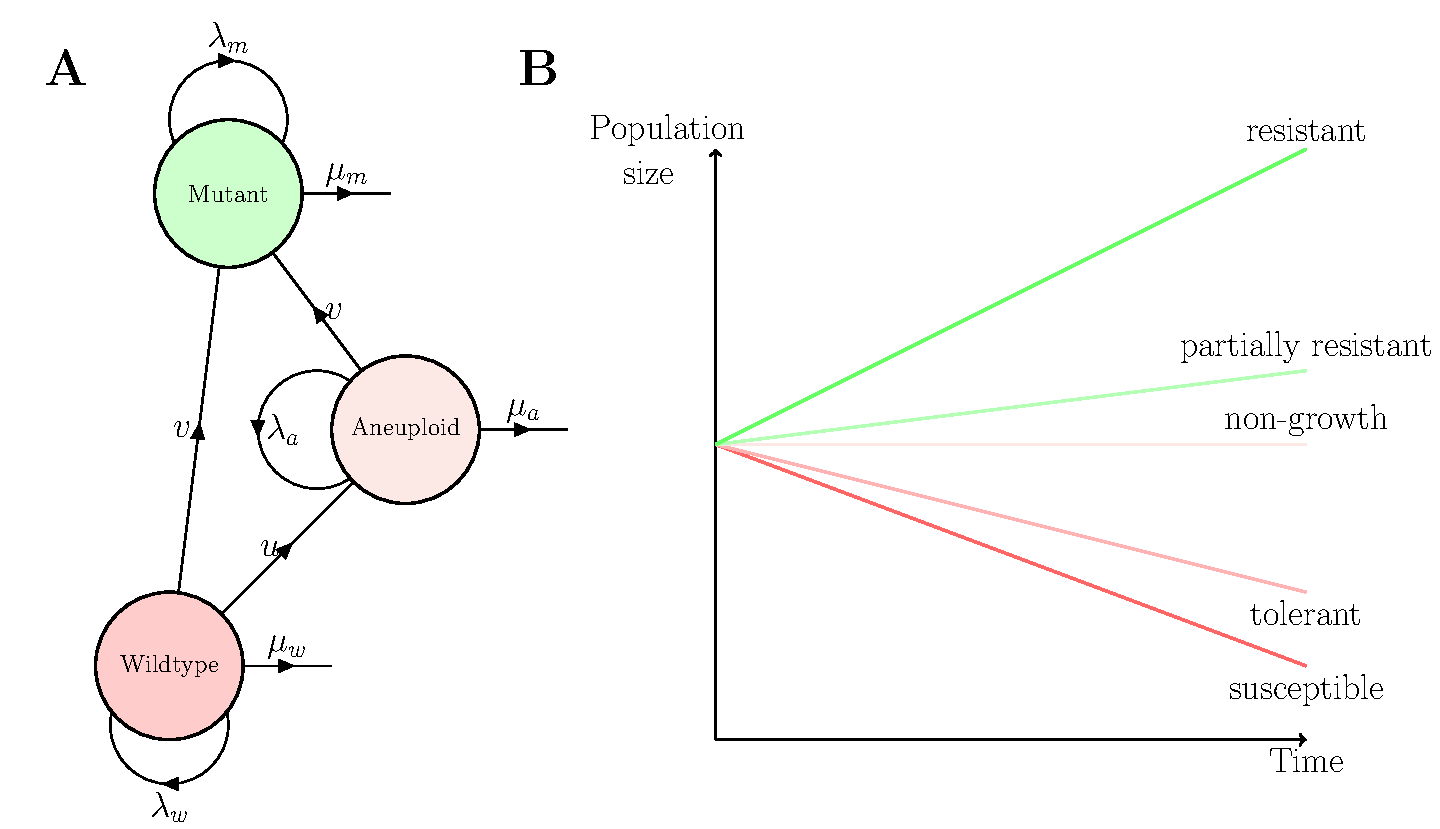
\includegraphics[width=\textwidth]{Figures/figureAneuploidy.pdf}
\caption{
\textbf{Model illustration.}
\textbf{(A)} A population of cancer cells is composed of drug-sensitive, aneuploid, and mutant cells, which divide with rates $\lambda_s$, $\lambda_a$, and $\lambda_m$ and die at rates $\mu_s$, $\mu_a$, and $\mu_m$, respectively. 
Sensitive cells can divide and become aneuploid at rate $u\lambda_s$. Both aneuploid and sensitive cells can divide and acquire a mutation with rates $v\lambda_a$ and $v\lambda_s$, respectively. Color denotes the relative growth rates of the three genotypes such that $\lambda_s - \mu_s < \lambda_a - \mu_a < \lambda_m - \mu_m$. \textbf{(B)} Sensitive cells are sensitive to the drug, while mutant cells are drug-resistant. The aneuploid may be tolerant, stationary, or partially resistant.
}
\label{figureAneuploidy}
\end{figure}

%%%%%%%%%%%
\begin{figure}
\begin{subfigure}{0.5\textwidth}
A\\
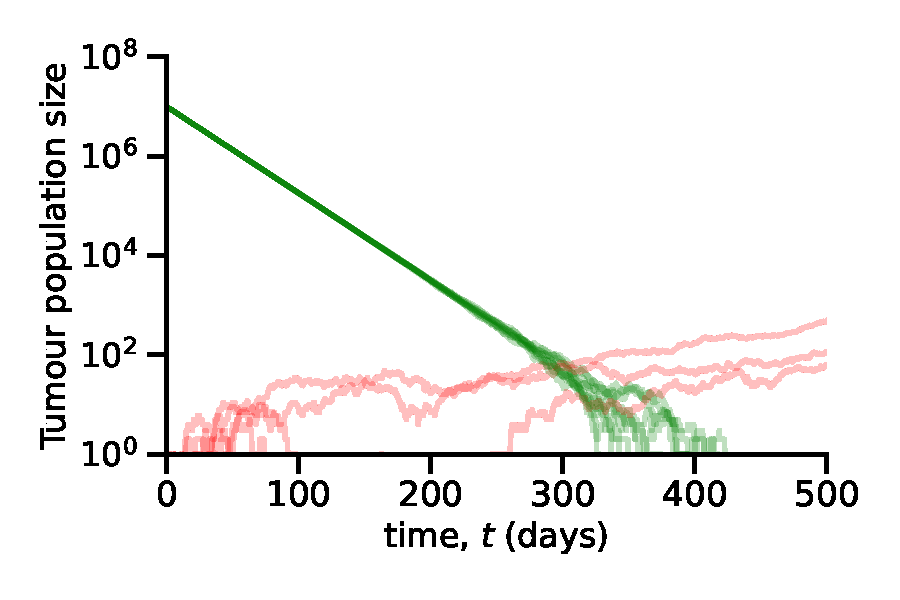
\includegraphics[width=1\textwidth]{Figures/TauLeapMeanTimeDiagramNoAneuploidy.pdf}
\end{subfigure}
\begin{subfigure}{0.5\textwidth}
B\\
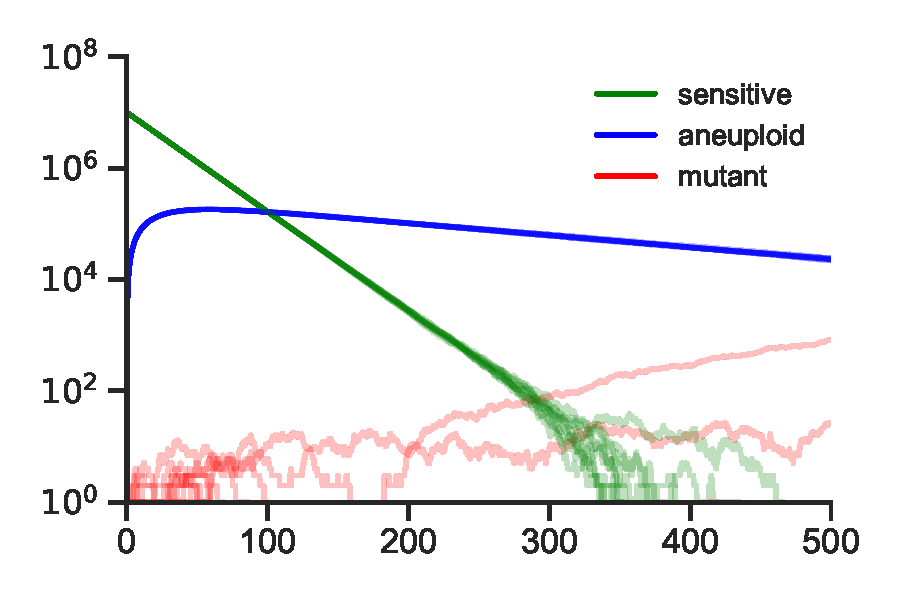
\includegraphics[width=1\textwidth]{Figures/TauLeapMeanTimeDiagramSmallda.pdf}
\end{subfigure}
\\
\begin{subfigure}{0.5\textwidth}
C\\
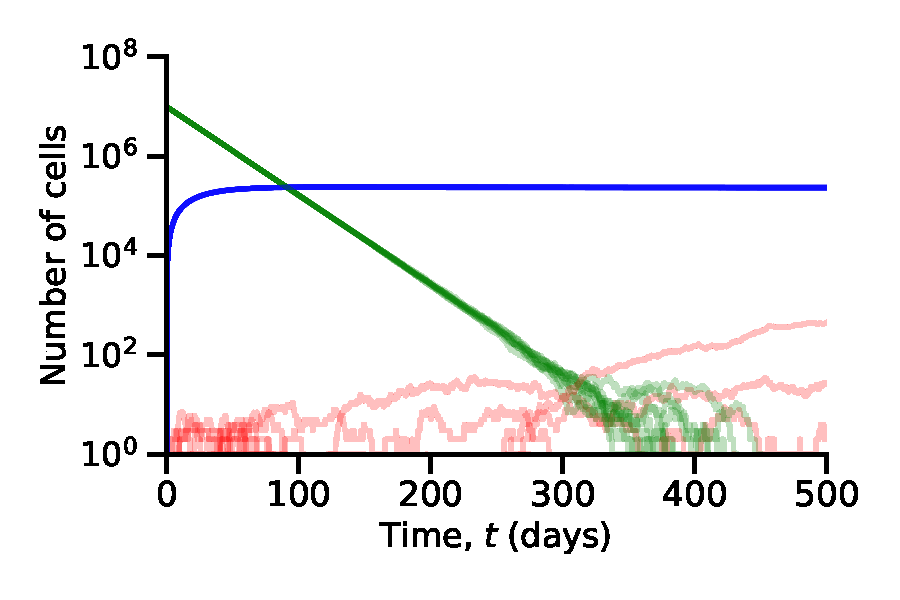
\includegraphics[width=1\textwidth]{Figures/TauLeapMeanTimeDiagramdazero.pdf}
\end{subfigure}
\begin{subfigure}{0.5\textwidth}
D\\
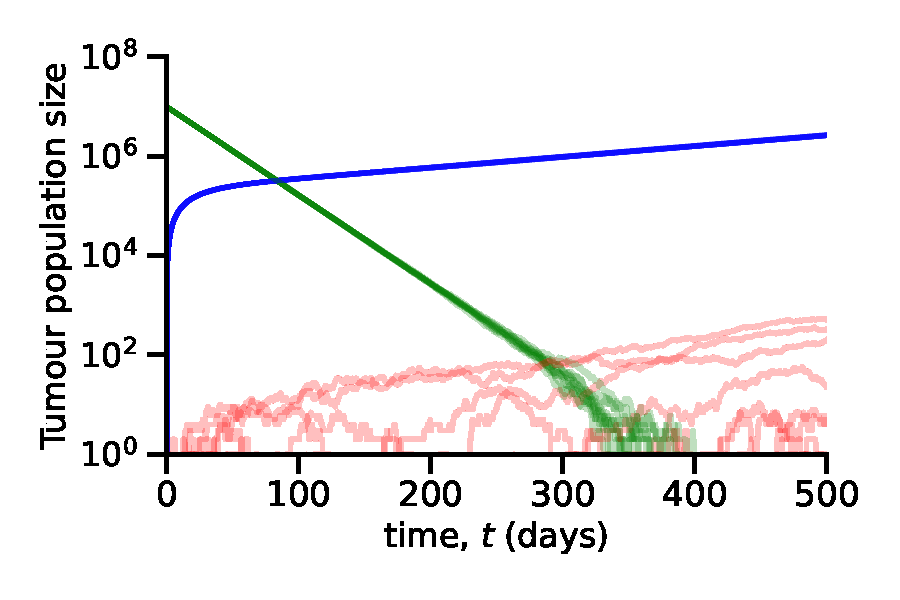
\includegraphics[width=1\textwidth]{Figures/TauLeapMeanTimeDiagramlargeda.pdf}
\end{subfigure}
\caption{
\textbf{Sample trajectories of the genotype frequencies.}
(A) Without aneuploidy ($u=0$), evolutionary rescue is possible through direct mutation, and in most scenarios, the tumor will become extinct due to the drug. (B) When aneuploid cells are tolerant ($\Delta_a<0$) evolutionary rescue can occur indirectly, but direct mutation is the most likely path for evolutionary rescue. %change 24
(C) When aneuploid cells are stationary ($\Delta_a\approx0$), we observe the appearance of mutant lineages even after the sensitive population has gone extinct, thus showing that stationary aneuploidy increases the probability of evolutionary rescue. (D) When aneuploid cells are partially resistant ($\Delta_a>0$), the tumor is rescued by the aneuploid cell population. Each plot shows 10 simulations of the number of sensitive, aneuploid, and mutant cells $\left(s_t,a_t,m_t\right)$ over time $t$.
Here, $\lambda_s=0.1$, $\lambda_m=0.1$, $\mu_s=0.14$, $\mu_a=0.09$, $\mu_m=0.09$, $v=10^{-7}$ , $N=10^7$; (A) $u=0$; (B) $\lambda_a=0.065$, $u=10^{-2}$; (C) $\lambda_a=0.08999$, $u=10^{-2}$; (D) $\lambda_a=0.095$, $u=10^{-2}$.
}
\label{sampleTrajectories}
\end{figure}

%%%%%%%%%%%
% Fig 3A: prob rescue vs N for various Delta_a; markup N*
% Fig 3B: N* vs Delta_a
% Fig 3C: N* vs u/v


\begin{figure}
\begin{subfigure}{0.48\textwidth}
A\\
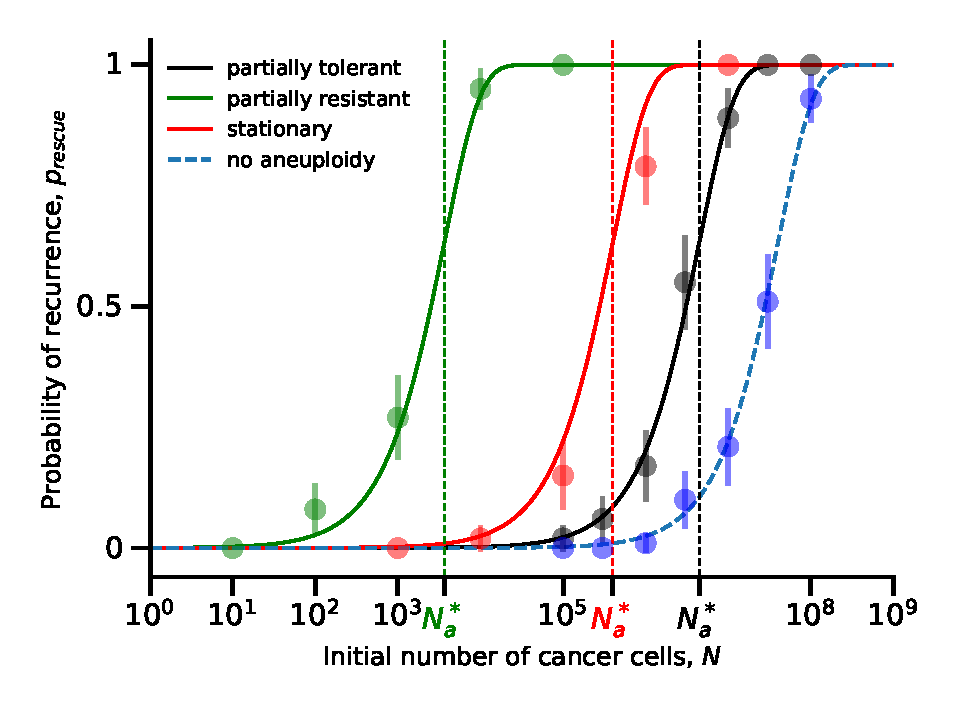
\includegraphics[width=1\textwidth]{Figures/ProbvNPlot.pdf}
\end{subfigure}
\begin{subfigure}{0.52\textwidth}
B\\
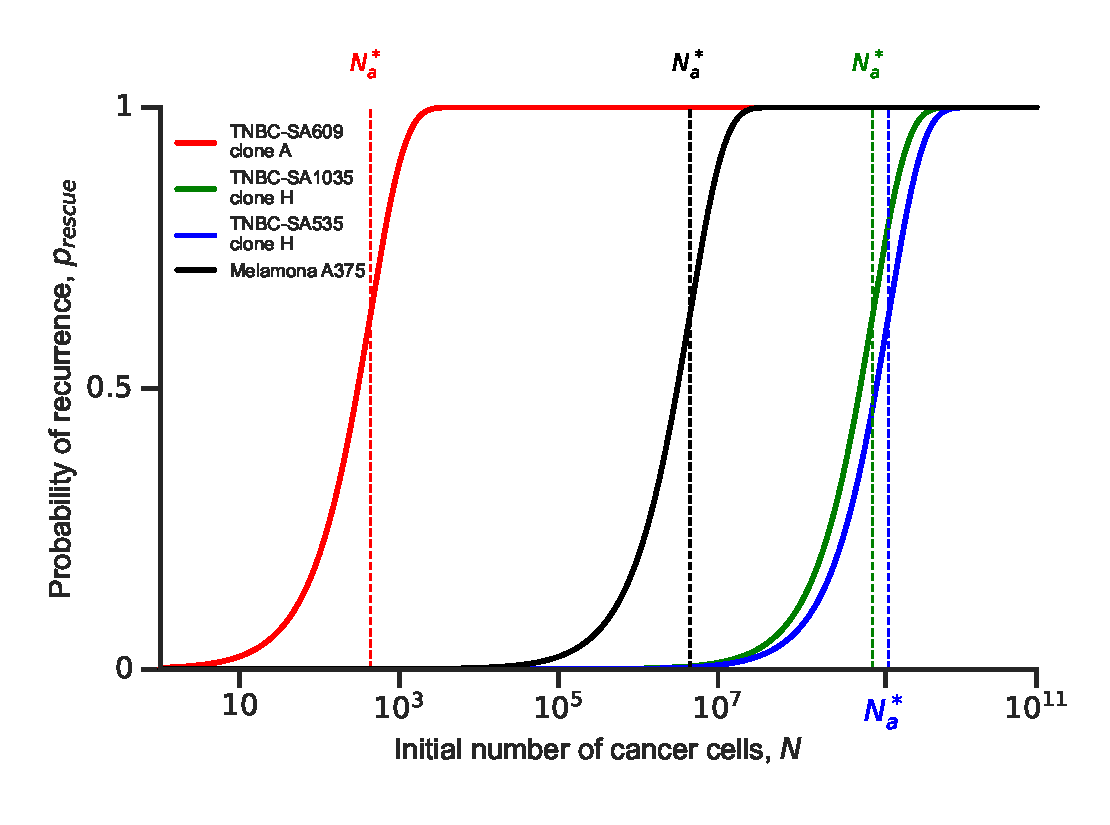
\includegraphics[width=1\textwidth]{Figures/PDXModelProb.pdf}
\end{subfigure}
\caption{\textbf{Aneuploidy facilitates the evolutionary rescue of cancer under drug treatment.}
The probability of evolutionary rescue, $\presc$, as a function of the initial tumor size, $N$ (\cref{eq:rescue_prob}). 
Dashed vertical lines show the threshold tumor size, $N_a^*$, above which the probability is very high (\cref{eq:N_a}). 
\textbf{(A)} Blue dashed line: without aneuploidy ($u=0$). Black line: tolerant aneuploidy ($u=10^{-2}, \lambda_a=0.0899$). Red line: stationary aneuploidy ($u=10^{-2}, \lambda_a=0.08999$). Green line: partially resistant aneuploidy ($u=10^{-2}, \lambda_a=0.095$). Markers and error bars for averages of simulation results with $95\%$ confidence interval ($p\pm1.96\sqrt{p\left(1-p\right)/n}$ where $p$ is the fraction of simulations in which the tumor has been rescued, and $n=100$ is the number of simulations). Parameters: $\lambda_s=0.1,\lambda_m=0.1,\mu_s=0.14,\mu_a=0.09,\mu_m=0.09, v=10^{-7}$.
\textbf{(B)} Comparison for melanoma and breast cancer with parameters from the literature (\Cref{table1,table2}). Black line: Melanoma A375. Blue line: Breast cancer TNBC-SA1035 clone H. Red line: Breast cancer TNBC-SA609 clone A. Green line: Breast cancer TNBC-SA535 clone H.
}
\label{rescue_prob}
\end{figure}

\begin{figure}
\begin{subfigure}{0.5\textwidth}
A\\
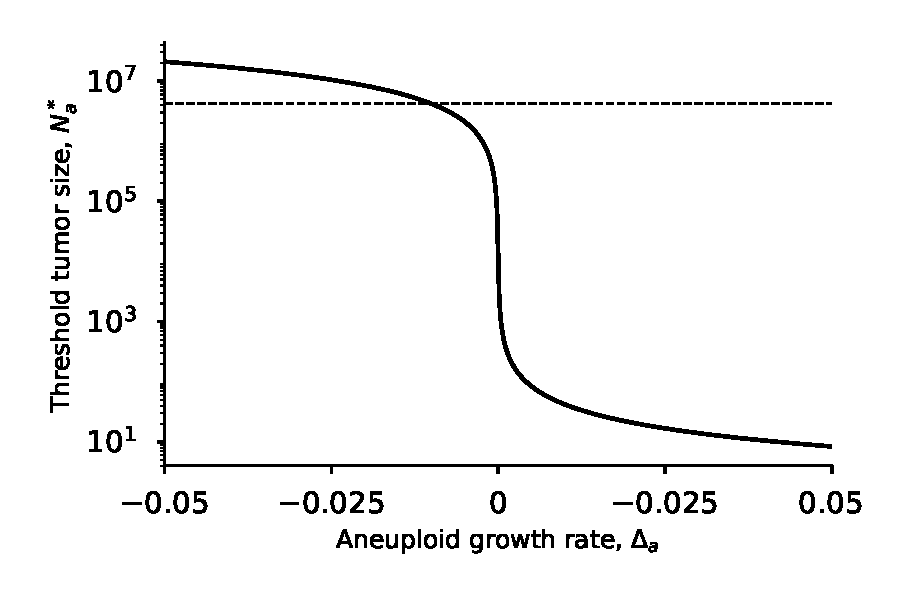
\includegraphics[width=1\textwidth]{Figures/ThresholdPopulationSizePlot.pdf}
\end{subfigure}
\begin{subfigure}{0.5\textwidth}
B\\
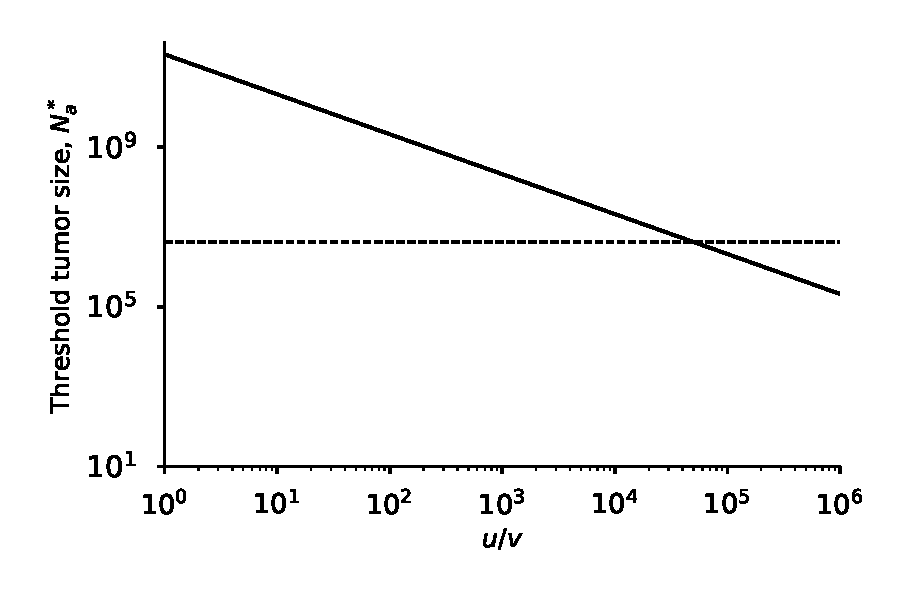
\includegraphics[width=1\textwidth]{Figures/ThresholdPopulationSizeVersusRatioPlot.pdf}
\end{subfigure}
\caption{
\textbf{The effect of aneuploidy on tumor threshold size.}
(A) The threshold tumor size $N_a^*$ (\cref{eq:N_a}) as a function of the aneuploid growth rate $\Delta_a$. The dashed horizontal line shows $N^*_m$ (\cref{eq:N_m}), the threshold tumor size without aneuploidy ($u=0$).  When aneuploid growth rate is close to or higher than zero, aneuploidy decreases the threshold tumor size, facilitating evolutionary rescue. The inset highlights the scenario when aneuploid cells are stationary. Red dots for simulations and error bars for the $95\%$ confidence intervals obtained with bootstrap (Appendix G). Parameters: $\lambda_s=0.1,\lambda_m=0.1,\mu_s=0.14,\mu_a=0.09,\mu_m=0.09, u=10^{-2}, v=10^{-7}$. %change 43
(B) Threshold tumor size $N_a^*$ (\cref{eq:N_a}) as a function of the ratio of aneuploidy and mutation rates, $u/v$. Dashed horizontal line shows $N^*_m$ (\cref{eq:N_m}), the threshold tumor size without aneuploidy ($u=0$). When the aneuploidy rate is much higher than the mutation rate, aneuploidy decreases the threshold tumor size, facilitating evolutionary rescue. Blue line represents the exact formula for threshold tumor size $N_a^*$ while the solid black line represents the approximation (\cref{eq:N_a}). Red dots represent simulation results, and the error bars represent the $95\%$ confidence intervals obtained with bootstrap (Appendix G).  Parameters: $\lambda_s=0.1,\lambda_a=0.0899,\lambda_m=0.1,\mu_s=0.14,\mu_a=0.09,\mu_m=0.09, v=10^{-7}$.  %change 18, 43
}
\label{rescue_threshold}
\end{figure}

%%%%%%%%%%%
% Fig 3A: N*/N* vs Delta_w 
% Fig 3B: N*/N* vs ut/s 

\begin{figure}
\begin{subfigure}{0.5\textwidth}
A\\
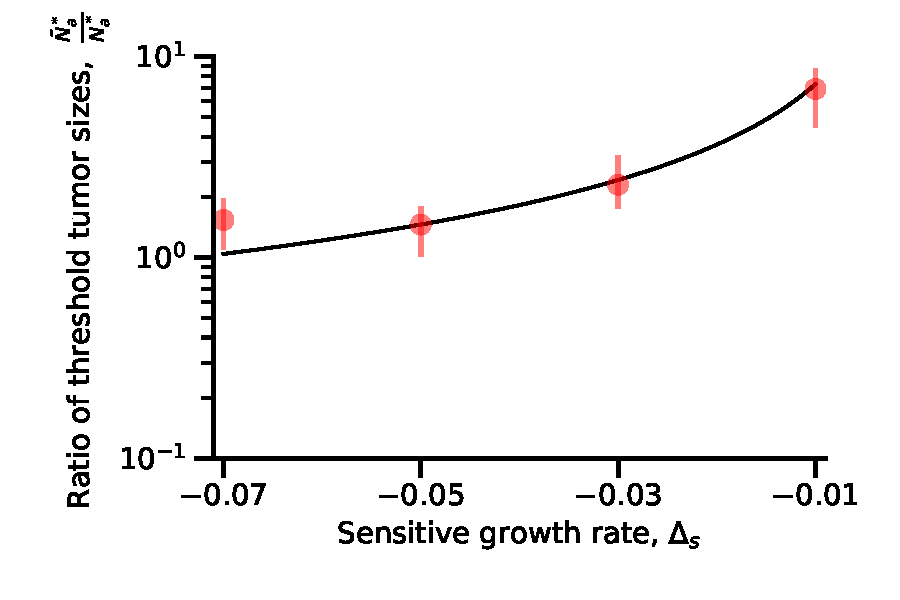
\includegraphics[width=1\textwidth]{Figures/RatiodsPlot.pdf}
\end{subfigure}
\begin{subfigure}{0.5\textwidth}
B\\
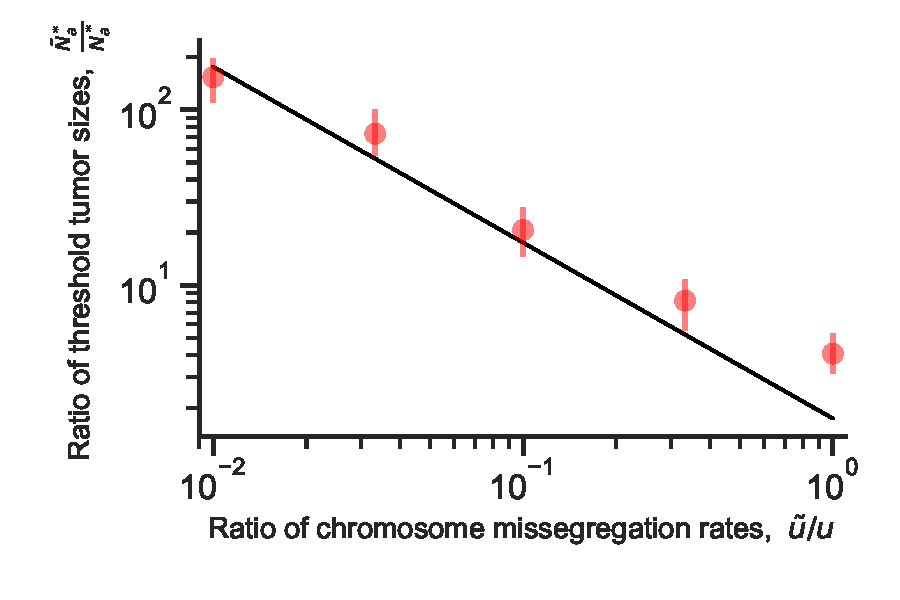
\includegraphics[width=1\textwidth]{Figures/ratio_uPlot.pdf}
\end{subfigure}
\caption{
\textbf{Standing genetic variation facilitates the evolutionary rescue of cancer.}
(A)  Ratio of threshold tumor sizes for rescue by standing genetic variation and by \textit{de novo} variation, $\tilde{N}_a^*/N_a^*$, when a fraction $\frac{\tilde{u}\lambda_s}{c}$ is aneuploid at the start of treatment, as a function of the sensitive growth rate $\Delta_s$.  Standing genetic variation will drive adaptation to the drug if the sensitive population is rapidly declining ($\Delta_s\ll0$) due to a stronger effect of the drug on sensitive cells. Red dots represent simulation results, and the error bars represent the $95\%$ confidence intervals obtained with bootstrap (Appendix G). Parameters: $\lambda_s=0.1,\lambda_a=0.0899,\lambda_m=0.1,\mu_a=0.09,\mu_m=0.09,\tilde{u}=10^{-3},u=10^{-2}, v=10^{-7}$.
(B) Ratio of threshold tumor size $\tilde{N}_a^*$, when a fraction $\frac{\tilde{u}\lambda_s}{c}$ is aneuploid at the start of treatment, and $N_a^*$ as a function of the ratio of aneuploidy rates $\tilde{u}/u$. \textit{De novo} aneuploids will have a larger contribution to the appearance of drug resistance if the drug induces the appearance of aneuploid cells ($u \gg \tilde u$). Red dots represent simulation results, and the error bars represent the $95\%$ confidence intervals obtained with bootstrap (Appendix G). Parameters: $\lambda_s=0.1,\lambda_a=0.0899,\lambda_m=0.1,\mu_s=0.14,\mu_a=0.09,\mu_m=0.09,\tilde{u}=10^{-3}, v=10^{-7}$.
}
\label{rescue_denovo}
\end{figure}
%%%%%%%%%%%


\begin{figure}
\vspace*{1\baselineskip}
\begin{subfigure}{0.5\textwidth}
A\\
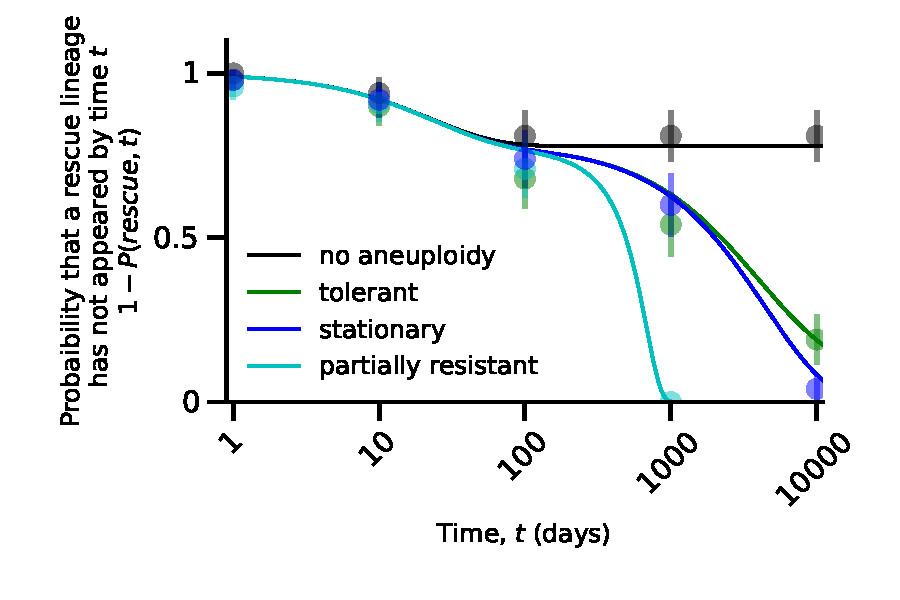
\includegraphics[width=1\textwidth]{Figures/ReboundProbability.pdf}
\end{subfigure}
\begin{subfigure}{0.5\textwidth}
B\\
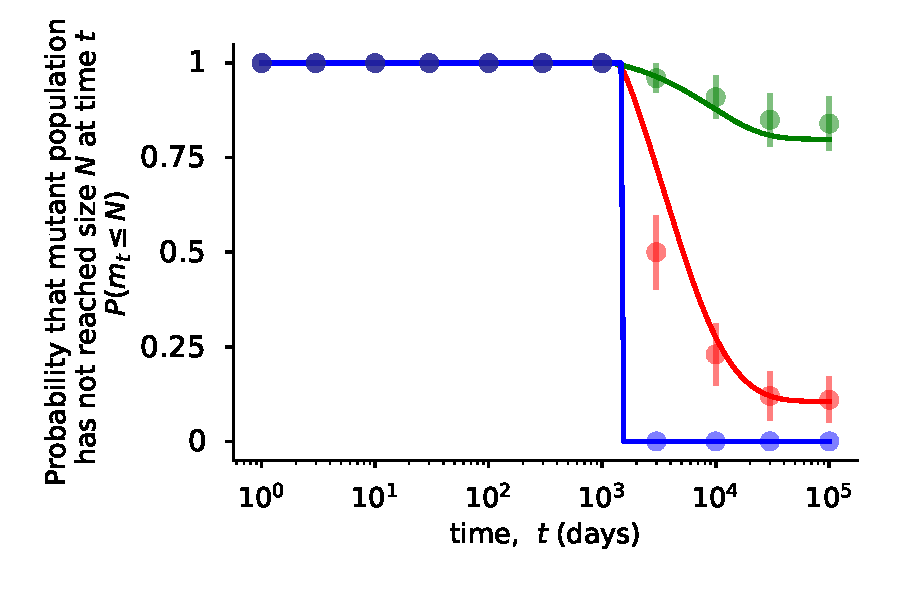
\includegraphics[width=1\textwidth]{Figures/ProliferationTimeCDFN.pdf}
\end{subfigure}
\caption{\textbf{Aneuploidy extends the window of opportunity for evolutionary rescue.}
(A) The probability that a successful mutant has not appeared by time $t$. Black line: tolerant aneuploidy ($u>0, \lambda_a=0.0899$). Red line: stationary aneuploidy ($u>0, \lambda_a=0.089999$). Green line: partially resistant aneuploidy ($u>0, \lambda_a=0.095$). Blue line: no aneuploidy ($u=0$). Aneuploidy plays an important role in rescuing the tumor cell population as the sensitive population becomes extinct. Markers represent simulation results, and the error bars represent $95\%$ confidence interval ($p\pm1.96\sqrt{p\left(1-p\right)/n}$ where $p$ is the fraction of simulations in which a successful mutant has not been generated, and $n=100$ is the number of simulations). Parameters: $\lambda_s=0.1,\lambda_m=0.1,\mu_s=0.14,\mu_a=0.09,\mu_m=0.09, u=10^{-2}, v=10^{-7},N=10^7$. %change 56
(B) Probability that a mutant cancer cell population has not reached size $N$ at time $t$ when aneuploidy provides tolerance. Green line: $N=10^6$ (small tumor). Red line: $N=10^7$ (intermediate-sized tumor). Blue line: $N=10^{10}$ (large tumor). Increasing the initial tumor size guarantees that the cancer will relapse. Markers represent simulations, and the error bars represent $95\%$ confidence interval ($p\pm1.96\sqrt{p\left(1-p\right)/n}$ where $p$ is the fraction of the simulations in which the mutant population size has not reached $N$ and $n=100$ is the number of simulations).
Parameters: $\lambda_s=0.1,\lambda_a=0.0899,\lambda_m=0.1,\mu_s=0.14,\mu_a=0.09,\mu_m=0.09, u=10^{-2}, v=10^{-7}$.}
\label{cdffig}
\end{figure}

%%%%%%%%%%%%%%%%%%%%%%%%%%%%%%%%%%%%%%%%%%

\begin{figure}
\vspace*{1\baselineskip}
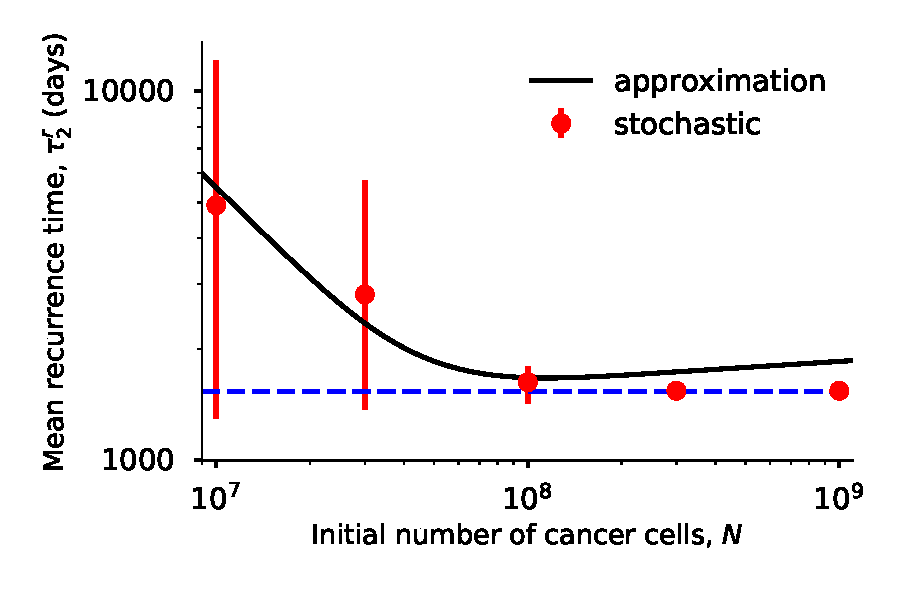
\includegraphics[width=1\textwidth]{Figures/ProliferationTime.pdf}
\caption{\textbf{Tumor size decreases the mean recurrence time.}
The mean time for the mutant cell population to reach size $N$, the initial number of cancer cells.
Our inhomogeneous Poisson-process approximation (solid black line, \cref{meanproliferationtime}) is in agreement with simulation results (red markers with error bars for 95\% CI) for intermediate size $N$.
Simulation results converge to \cref{eq:t2det} (blue dashed line) for large values of $N$. The green line represents the numerical solution of \cref{eq:t2det2024}. % change 44  
Parameters: $\lambda_s=0.1,\lambda_a=0.0899,\lambda_m=0.1,\mu_s=0.14,\mu_a=0.09,\mu_m=0.09, u=10^{-2}, v=10^{-7}$.}
\label{proliferationFigure}
\end{figure}


%%%%%%%%%%%%%%%%%%%%%%%%%%%%%%%%%%%%%

\newpage 

\begin{appendices}
\renewcommand{\theequation}{\thesection\arabic{equation}}
\counterwithin*{equation}{section}


%%%%%%%%%%%%%%%%%%%%%%%%%%%%%%%%%%%%%
\section{Survival probability of a single lineage}\label{sec:appendix-surv-prob}

To analyze evolutionary rescue in our model, we use the framework of \emph{multi-type branching processes} \citep{harris1963theory, weissman2009rate}. 
In the case of cancer, where all reproduction is binary fission, these branching processes are also \emph{birth-death processes} \citep{kendall1948}% change 31
This allows us to find explicit expressions for the \emph{survival probability}: the probability that a lineage descended from a single cell does not become extinct.

Let $p_s$, $p_a$, and $p_m$ be the survival probabilities of a population consisting initially of single sensitive cell, aneuploid cell, or mutant cell, respectively.
The complements $1-p_s$, $1-p_a$, and $1-p_m$ are the extinction probabilities, which satisfy each its respective equation~\citep{harris1963theory},
\begin{equation} \label{eq:extinction_prob}
\begin{aligned}
1-p_s = &\frac{\mu_s}{\lambda_s+\mu_s+u\lambda_s+v\lambda_s} + 
		  \frac{u\lambda_s}{\lambda_s+\mu_s+u\lambda_s+v\lambda_s}\left(1-p_a\right)\left(1-p_s\right) + \\
		  & \frac{\lambda_s}{\lambda_s+\mu_s+u\lambda_s+v\lambda_s}\left(1-p_s\right)^2 +
		  \frac{v\lambda_s}{\lambda_s+\mu_s+u\lambda_s+v\lambda_s}\left(1-p_m\right)\left(1-p_s\right) ,\\
1-p_a = &\frac{\mu_a}{\lambda_a+\mu_a+v\lambda_a}+\frac{v\lambda_a}{\lambda_a+\mu_a+v\lambda_a}\left(1-p_m\right)\left(1-p_a\right)+\frac{\lambda_a}{\lambda_a+\mu_a+v\lambda_a}\left(1-p_a\right)^2 ,\\
1-p_m = &\frac{\mu_m}{\lambda_m+\mu_m}+\frac{\lambda_m}{\lambda_m+\mu_m}\left(1-p_m\right)^2 .	 
\end{aligned}
\end{equation}

The survival probabilities are given by the smallest solution for each quadratic equation \citep{uecker2015adaptive}. Therefore we have
\begin{equation}\label{eq:survival_prob}
\begin{aligned}
p_s &= \frac{\lambda_s-\mu_s-u\lambda_sp_a-v\lambda_sp_m+\sqrt{\left(\lambda_s-\mu_s-u\lambda_sp_a-v\lambda_sp_m\right)^2+4\lambda_s^2\left(up_a+vp_m\right)}}{2\lambda_s} ,\\
p_a &= \frac{\lambda_a-\mu_a-v\lambda_ap_m+\sqrt{\left(\lambda_a-\mu_a-v\lambda_ap_m\right)^2+4\lambda_a^2vp_m}}{2\lambda_a}, \\
p_m &= \frac{\lambda_m-\mu_m}{\lambda_m} .
\end{aligned} 
\end{equation}
Note that the equation for $p_s$ depends on both $p_a$ and $p_m$, and the equation for $p_a$ depends on $p_m$.
To proceed, we can plug the solution for $p_m$ and $p_a$ into the solution for $p_s$. We perform this for three different scenarios.

%%%%%%%%%%%%%%%%%%%%%%%%%%%%%%%%%%%%%
\subsubsection*{Scenario 1: Aneuploid cells are partially resistant} 

We first assume that aneuploidy provides partial resistance to drug therapy, $\lambda_a>\mu_a$, and that this resistance is significant, $\left(\lambda_a-\mu_a-v\lambda_ap_m\right)^2 > 4\lambda_a^2 v p_m$.
We thus rewrite \cref{eq:survival_prob} as
\begin{align*}
p_s&=\frac{\lambda_s-\mu_s-u\lambda_sp_a-v\lambda_sp_m}{2\lambda_s}\left(1-\sqrt{1+\frac{4\lambda_s^2\left(vp_m+up_a\right)}{\left(\lambda_s-\mu_s-u\lambda_sp_a-v\lambda_sp_m\right)^2}}\right) ,
\text{and} \\
p_a&=\frac{\lambda_a-\mu_a-v\lambda_ap_m}{2\lambda_a}\left(1+\sqrt{1+\frac{4\lambda_a^2vp_m}{\left(\lambda_a-\mu_a-v\lambda_ap_m\right)^2}}\right) . 
\end{align*}
Using the Taylor expansion $\sqrt{1+x}=1+x/2+\mathcal{O}(x^2)$ and assuming $u,v \ll 1$,
we obtain the following approximation for the survival probability of a population initially consisting of a single sensitive cell,
\begin{align} \label{eq:survprobwapprox1}
p_s
&\approx -\frac{v\lambda_sp_m+u\lambda_sp_a}{\lambda_s-\mu_s-u\lambda_sp_a-v\lambda_sp_m}\\
\nonumber
&\approx-\frac{1}{\lambda_s-\mu_s}\left[\frac{u\lambda_s\left(\lambda_a-\mu_a\right)}{\lambda_a}+\frac{uv\lambda_s\lambda_a\left(\lambda_m-\mu_m\right)}{\lambda_m\left(\lambda_a-\mu_a\right)}+\frac{v\lambda_s\left(\lambda_m-\mu_m\right)}{\lambda_m}\right].
\end{align}
Now $u v$ is very small, and if we use the fact that $v \ll u$, we have:
\begin{equation}\label{eq:pw_parttolerant}
p_s \approx \frac{u\lambda_s}{\abs{\Delta_s}}  \frac{\Delta_a}{\lambda_a} .
\end{equation}
However, if aneuploidy is very rare such that
\begin{align*}
\frac{u\lambda_s\Delta_a}{\lambda_a}<\frac{v\lambda_s\Delta_m}{\lambda_m}\Rightarrow u\lambda_a<\frac{v\lambda_a^2\Delta_m}{\lambda_m} \frac{1}{\Delta_a}<\frac{v\lambda_a^2\Delta_m}{\lambda_m} \frac{1}{\sqrt{4\lambda_a^2 v p_m}}\Rightarrow u\lambda_a<T^*,
\end{align*}
where $T^* = (4 v \lambda_a^2 \Delta_m/\lambda_m)^{-1/2}$ and in the second inequality we used the fact that $\Delta_a^2 > 4\lambda_a^2 v p_m$. In this scenario adaptation is through direct mutation and:
\begin{equation*}
p_s \approx \frac{v\lambda_s}{\abs{\Delta_s}}  \frac{\Delta_m}{\lambda_m} .
\end{equation*}
%%%%%%%%%%%%%%%%%%%%%%%%%%%%%%%%%%%%%
\subsubsection*{Scenario 2: Aneuploid cells are tolerant.} 

We now assume that aneuploidy provides tolerance to drug therapy, that is, the number of aneuploid cells significantly declines over time, but at a lower rate than the number of sensitive cells, $\lambda_s - \mu_s < \lambda_a - \mu_a < 0$. We also assume that the decline is significant, $\left(\lambda_a-\mu_a-v\lambda_ap_m\right)^2 > 4\lambda_a^2 v p_m$. %change 19
We rewrite \cref{eq:survival_prob} as
\begin{equation}
\begin{aligned}
p_s&=\frac{\lambda_s-\mu_s-u\lambda_sp_a-v\lambda_sp_m}{2\lambda_s}\left(1-\sqrt{1+\frac{4\lambda_s^2\left(vp_m+up_a\right)}{\left(\lambda_s-\mu_s-u\lambda_sp_a-v\lambda_sp_m\right)^2}}\right), \\
p_a&=\frac{\lambda_a-\mu_a-v\lambda_ap_m}{2\lambda_a}\left(1-\sqrt{1+\frac{4\lambda_a^2vp_m}{\left(\lambda_a-\mu_a-v\lambda_ap_m\right)^2}}\right) .
\end{aligned}
\end{equation}
Since $u,v\ll1$, the term in the root can be approximated using a Taylor expansion. So, substituting the expressions for $p_a$ and $p_m$, we have
\begin{equation} \label{eq:survprobwinitial}
\begin{aligned}
p_s&\approx-\frac{v\lambda_sp_m+u\lambda_sp_a}{\lambda_s-\mu_s-u\lambda_sp_a-v\lambda_sp_m}\\
&\approx\frac{1}{\lambda_s-\mu_s-u\lambda_sp_a-v\lambda_sp_m}\left[\frac{uv\lambda_s\lambda_a\left(\lambda_m-\mu_m\right)}{\lambda_m\left(\lambda_a-\mu_a-v\lambda_a\right)}-\frac{v\lambda_s\left(\lambda_m-\mu_m\right)}{\lambda_m}\right]\\ 
&\approx\frac{v\lambda_s\left(\lambda_m-\mu_m\right)}{\lambda_m\left(\lambda_s-\mu_s\right)}\left[\frac{u\lambda_a}{\left(\lambda_a-\mu_a\right)}-1\right] \\
&=\frac{v\lambda_s\Delta_m}{\lambda_m \abs{\Delta_s}}\left(\frac{u\lambda_a}{\abs{\Delta_a}}+1\right) .
\end{aligned}
\end{equation}
If we assume that aneuploidy is not rare ($u\lambda_a>\abs{\Delta_a}$) then we have:
\begin{equation}\label{eq:pw_tolerant}
p_s\approx\frac{u\lambda_s}{\abs{\Delta_s}} \frac{v\lambda_a}{\abs{\Delta_a}} \frac{\Delta_m}{\lambda_m}.
\end{equation}

%%%%%%%%%%%%%%%%%%%%%%%%%%%%%%%%%%%%%
\subsubsection*{Scenario 3: Aneuploid cells are stationary} 
We now assume that the growth rate of aneuploid cells is close to zero (either positive or negative), such that  $\left(\Delta_a-v\lambda_ap_m\right)^2 \ll 4\lambda_a^2vp_m$.
We rewrite \cref{eq:survival_prob} as
\begin{equation}
p_a = \frac{\lambda_a-\mu_a-v\lambda_ap_m+2\sqrt{\lambda_a^2 vp_m}\left(1+\frac{\left(\lambda_a-\mu_a-v\lambda_ap_m\right)^2}{4\lambda_a^2vp_m}\right)^{\frac12}}{2\lambda_a} .
\end{equation}
Using a following Taylor series expansion for small $\left(\lambda_a-\mu_a-v\lambda_ap_m\right)^2 / 4\lambda_a^2vp_m$,
\begin{equation*}
\left(1+\frac{\left(\lambda_a-\mu_a-v\lambda_ap_m\right)^2}{4\lambda_a^2vp_m}\right)^{\frac{1}{2}}=1+\frac{\left(\lambda_a-\mu_a-v\lambda_ap_m\right)^2}{8\lambda_a^2vp_m}+\cdots,
\end{equation*}
we obtain the approximation
\begin{equation}
\begin{aligned}
p_a&\approx\frac{\lambda_a-\mu_a-v\lambda_ap_m+2\sqrt{\lambda_a^2 vp_m}\left[1+\frac{\left(\lambda_a-\mu_a-v\lambda_ap_m\right)^2}{8\lambda_a^2vp_m}\right]}{2\lambda_a}\\
&=\frac{\lambda_a-\mu_a-v\lambda_ap_m+2\sqrt{\lambda_a^2 vp_m}+\frac{\left(\lambda_a-\mu_a-v\lambda_ap_m\right)^2}{4\sqrt{\lambda_a^2vp_m}}}{2\lambda_a}\\
&=\frac{\left(\lambda_a-\mu_a-v\lambda_ap_m+2\sqrt{\lambda_a^2vp_m}\right)^2+4\lambda_a^2vp_m}{8\lambda_a\sqrt{\lambda_a^2vp_m}}\\
&=\frac{4\lambda_a^2vp_m+4\lambda_a^2vp_m\left(1+\frac{\lambda_a-\mu_a-v\lambda_ap_m}{2\sqrt{\lambda_a^2vp_m}}\right)^2}{8\lambda_a\sqrt{\lambda_a^2vp_m}}\\
&=\frac{1}{2\lambda_a}\left(\lambda_a-\mu_a-v\lambda_ap_m+2\sqrt{\lambda_a^2vp_m}\right).
\end{aligned}
\end{equation}
Plugging this in \cref{eq:survprobwapprox1}, the survival probability of a population starting from one sensitive cell is
\begin{equation}\label{eq:scenario3}
\begin{aligned}
p_s&\approx-\frac{1}{\lambda_s-\mu_s-u\lambda_sp_a-v\lambda_sp_m}\left[v\lambda_s\frac{\lambda_m-\mu_m}{\lambda_m}+\frac{u\lambda_s}{2\lambda_a}\left(\lambda_a-\mu_a-v\lambda_ap_m+2\sqrt{\lambda_a^2vp_m}\right)\right]\\
&=-\frac{1}{\lambda_s-\mu_s-u\lambda_sp_a-v\lambda_sp_m}\left[v\lambda_s\frac{\lambda_m-\mu_m} {\lambda_m}+\frac{u\lambda_s}{2\lambda_a}\left(\lambda_a-\mu_a-v\lambda_ap_m\right)+u\lambda_s\sqrt{\frac{v\left(\lambda_m-\mu_m\right)}{\lambda_m}}\right]\\ %change 20
&\approx-\frac{1}{\Delta_s}\left[v\lambda_s\frac{\Delta_m}{\lambda_m}+\frac{u\lambda_s\left(\Delta_a-v\lambda_ap_m\right)}{2\lambda_a}+u\lambda_s\sqrt{\frac{v\Delta_m}{\lambda_m}}\right]. %change 21
\end{aligned}
\end{equation}
Using the fact that
\begin{equation*}
\left(\Delta_a-v\lambda_ap_m\right)^2 \ll 4\lambda_a^2vp_m\Rightarrow\frac{\Delta_a-v\lambda_ap_m}{2\lambda_a} \ll \sqrt{\frac{v\lambda_a\Delta_m}{\lambda_m}},
\end{equation*}
and $v\ll u$ we obtain:
\begin{equation}\label{eq:pw_partrest}
p_s\approx\frac{u\lambda_s}{\abs{\Delta_s}} \sqrt{\frac{v\lambda_a\Delta_m}{\lambda_m}}.
\end{equation}
%%%%%%%%%%%%%%%%%%%%%%%%%%%%%%%%%%%%%%%%%%

\section{Evolutionary rescue probability}\label{sec:appendix-rescue-prob}
Using the fact that $\Delta_a-v\lambda_ap_m\approx\Delta_a$ we write the condition $\left(\Delta_a-v\lambda_ap_m\right)^2 \ll 4\lambda_a^2vp_m$ as:
\begin{equation*}
\Delta_a^2 \ll 4\lambda_a^2vp_m\Rightarrow -1\ll\Delta_aT^*\ll1,
\end{equation*}
where $T^* = (4 v \lambda_a^2 \Delta_m/\lambda_m)^{-1/2}$.
Substituting \cref{eq:pw_parttolerant,eq:pw_partrest,eq:pw_tolerant} into \cref{eq:rescue_prob}, the evolutionary rescue probability can be approximated by
\begin{equation}\label{rescue_prob_approx}
\begin{aligned}
&\presc \approx \\
  &\begin{cases}
   1-\exp\left[-\frac{u\lambda_a}{\abs{\Delta_s}} \frac{v\lambda_s}{\abs{\Delta_a}} \frac{\Delta_m}{\lambda_m}  N\right] ,&
   \Delta_aT^*\ll-1 ,\\
   1-\exp\left[-\frac{u\lambda_s}{\abs{\Delta_s}} \sqrt{\frac{v\lambda_a\Delta_m}{\lambda_m}} N\right] ,&
  -1\ll\Delta_aT^*\ll1 ,\\
   1-\exp\left[-\frac{u\lambda_s}{\abs{\Delta_s}}  \frac{\Delta_a}{\lambda_a}  N\right] ,&
   1\ll\Delta_aT^*.
  \end{cases}
\end{aligned}
\end{equation}
%%%%%%%%%%%%%%%%%%%%%%%%%%%%%%%%%%%%%%%%%%

\section{Evolutionary rescue time}\label{sec:appendix_rescue_time}

We first calculate the expected time for the appearance of the first mutant that rescues the cell population.
This can occur either through the evolutionary trajectory \textit{sensitive}$\rightarrow$\textit{mutant} or through the trajectory \textit{sensitive}$\rightarrow$\textit{aneuploid}$\rightarrow$\textit{mutant}.
We start with the former. 

Assuming no aneuploidy ($u=0$), we define $T_m$ to be the time at which the first mutant cell appears that will avoid extinction and will therefore rescue the population.
Note that if extinction occurs, that is the frequency of mutants after a very long time is zero, $m_{\infty}=0$, then it is implied that $T_m=\infty$, and vice versa if $T_m<\infty$ then $m_{\infty}>0$.

The number of successful mutants generated until time $t$ can be approximated by an inhomogeneous Poisson process with rate $R_m\left(t\right) = v\lambda_s p_m s_t$, %change 7
where $s_t=N\e^{\Delta_s t}$ is the number of sensitive cells at time $t$.
Note that 
\begin{equation}\label{eq:integralR}
\int_0^{t}{R_m(z)\d z} = 
v\lambda_s p_m N \frac{\exp[{\Delta_s t}]-1}{\Delta_s} \approx 
v\lambda_s p_m N t,
\end{equation}
by integrating the exponential and because $\frac{1}{\Delta_s} \left(\exp[\Delta_s t]-1\right) = t+ \bigo{\Delta_s t^2}$. %change 22
The probability density function of $T_m$ is thus
$R_m\left(t\right)\exp\left(-\int_0^{t}{R_m(z)\d z}\right)$ \citep{allen2010introduction}. 
Therefore, the probability density function of the conditional random variable $(T_m \mid T_m < \infty)$ is
$f_m(t) = R_m \left(t\right)\exp\left(-\int_0^{t}{R_m(z)\d z}\right) / \presc$. 
\\

We are interested in the mean conditional time, $\tau_m=\mathbb{E}\left[T_m \mid T_m<\infty\right]$, which is given by
\begin{equation}\label{eq:meantime1}
\begin{aligned}
\tau_m =
\int_{0}^{\infty}{t f_m(t) \d t} = 
\frac{\int_{0}^{\infty}{tR_m(t)\exp\left(-\int_0^{t}{R_m(z)\d z}\right) \d t}}{\presc},
\end{aligned}
\end{equation}
Therefore, plugging \cref{eq:integralR,eq:rescue_prob} in \cref{eq:meantime1}, 
\begin{align}\label{eq:limitapprox_appendix}
\tau_m = 
\int_0^\infty tv\lambda_s N\e^{\Delta_st}\frac{\e^{-v\lambda_s N p_m\frac{\e^{\Delta_s t}-1}{\Delta_s}} }{1-\left(1-p_s\right)^N} \d t\approx
\int_{0}^{\infty} tv\lambda_s N\e^{\Delta_st}\frac{\e^{-v\lambda_s N p_mt} }{1-\e^{-Np_s}}\d t. 
\end{align}
\Cref{MeanTimeGrowthAneuploidyPlot}B shows the agreement between this approximation and simulation results. %change  8
\\
Assuming aneuploidy is possible ($u>0$), we define $T_a$ to be the time at which the first mutant cell appears that will rescue the population. We are interested in the mean conditional time, $\tau_a=\mathbb{E}\left[T_a \mid T_a<\infty\right]$.

When $Nu\lambda_s/\abs{\Delta_s}\gg1$ the aneuploid frequency dynamics is roughly deterministic and therefore can be approximated by 
\begin{equation}\label{aneuploidpopeq}
a_t \approx \frac{Nu\lambda_s}{\Delta_s-\Delta_a}\left(\e^{\Delta_st}-\e^{\Delta_a t}\right).
\end{equation}
As a result, the number of successful mutants created by direct mutation and via aneuploidy can be approximated by inhomogeneous Poisson processes with the rates
\begin{align*}
n_1\left(t\right)&=v\lambda_ap_ma_{t},\\
r_2\left(t\right)&=v\lambda_sp_ms_{t},
\end{align*}
and the expected number of successful mutants created by direct mutation and via aneuploidy until time $t$ is given by:
\begin{align}
M_a\left(t\right)&=v\lambda_ap_m\int_0^ta_{z} d z = \frac{uv\lambda_s\lambda_aNp_m}{\Delta_s-\Delta_a}\left(\frac{\e^{\Delta_st}-1}{\Delta_s}-\frac{\e^{\Delta_at}-1}{\Delta_a}\right),\label{eq:twosteplineage}\\ 
M_m\left(t\right)&=v\lambda_sp_m\int_0^ts_{z} d z = v\lambda_sNp_m\frac{\e^{\Delta_s t}-1}{\Delta_s}.\label{eq:twosteplineagedirect}
\end{align} %change r3

For large initial population sizes we assume that the two processes are independent and as a result, they can be merged into a single Poisson process with rate $R_a(t)=\left(n_1+r_2\right)\left(t\right)$.
Consequently, the mean time to the appearance of the first rescue mutant is
\begin{align}\nonumber
\tau_a &= \frac{\int_{0}^{\infty}{tR_a(t)\exp\left(-\int_0^{t}{R_a(z)\d z}\right) \d t}}{\presc}\\ \label{meantimet2}
&=
\int_0^\infty t\left(v\lambda_ap_ma_t+v\lambda_sp_ms_t\right)\frac{\exp\left[-\frac{uv\lambda_s\lambda_aNp_m}{\Delta_s-\Delta_a}\left(\frac{\e^{\Delta_s t}-1}{\Delta_s}-\frac{\e^{\Delta_a t}-1}{\Delta_a}\right)-v\lambda_sNp_m\frac{\e^{\Delta_s t}-1}{\Delta_s}\right] }{1-\e^{-Np_s}}\d t,
\end{align}
which we plot in \Cref{MeanTimeGrowthAneuploidyPlot}A as a function of the initial population size, $N$.

Paradoxically, we observe from \Cref{MeanTimeGrowthAneuploidyPlot} that the mean time of a rescue mutation to appear is significantly shorter for the scenario when $u=0$ when compared to the scenario $u>0$, however this can be explained by the fact this mean time is conditioned on evolutionary rescue and, as a result, aneuploidy increase the \emph{window of opportunity} in which a rescue mutation could appear thus increasing the mean time as well (\Cref{sampleTrajectories}).

%%%
Let $N_a^*$ and $N_m^*$ be the threshold population size above which evolutionary rescue through aneuploidy or direct mutation, respectively, is very likely. The mean time $\tau_a$ can be written as: % change 38
\begin{align*}
\tau_a&=\int_0^\infty tf(t)dt=\int_0^\infty t\frac{d}{dt}F(t)dt=-\int_0^\infty t\frac{d}{dt}S(t)dt\\
&=-\left[tS(t)\right]_0^\infty+\int_0^\infty S(t)dt\\
&=\int_0^\infty S(t)dt,
\end{align*}
where $f(t)$, $F(t)$ and $S(t)$ are the probability density function, cumulative distribution function and survival function.
In our case, $S(t)=\exp\left(-\int_0^t R_a(z)dz\right)$.
Additionally, for $N\gg N_m^*$ we have $1-\e^{-Np_s}\approx1$ and, as a result, we have: %change 23
\begin{align*}
\tau_a=\int_0^\infty\e^{-\int_0^t R_a\left(z\right)\d z}\,\d t=\int_0^\infty\exp\left[-\frac{uv\lambda_s\lambda_aNp_m}{\Delta_s-\Delta_a}\left(\frac{\e^{\Delta_s t}-1}{\Delta_s}-\frac{\e^{\Delta_a t}-1}{\Delta_a}\right)-v\lambda_sNp_m\frac{\e^{\Delta_s t}-1}{\Delta_s}\right]\,\d t,
\end{align*} %change r4
and we use the following Taylor series expansions:
\begin{align*}
\frac{\e^{\Delta_s t}-1}{\Delta_s}&=\frac{1+\Delta_s t+O(t^2)-1}{\Delta_s}=t+O(t^2).\\ % change r4
\frac{\e^{\Delta_a t}-1}{\Delta_a}&=\frac{1+\Delta_a t+O(t^2)-1}{\Delta_a}=t+O(t^2), % change r4
\end{align*}
to obtain a simpler approximation for $\tau_a$:
\begin{align}\label{limitapprox3}
\tau_a\approx\int_0^\infty\e^{-v\lambda_sNp_m t}\,\d t=\frac{1}{v\lambda_sNp_m}. % change r4
\end{align}
If $N\ll N_a^*$ then the probability distribution of evolutionary rescue time is skewed toward small values (i.e. evolutionary rescue occurs conditioned on it happening). As a result, we have: 
\begin{align*}
\frac{\e^{\Delta_s t}-1}{\Delta_s}&=\frac{1+\Delta_s t+\mathcal{O}\left(\left(\Delta_st\right)^2\right)-1}{\Delta_s}=t+\mathcal{O}\left(\Delta_st^2\right)\\
\frac{\e^{\Delta_a t}-1}{\Delta_a}&=\frac{1+\Delta_a t+\mathcal{O}\left(\left(\Delta_at\right)^2\right)-1}{\Delta_a}=t+\mathcal{O}\left(\Delta_at^2\right)
\end{align*}
We observe that the first term in the exponential in \cref{meantimet2} can be approximated to be zero and the second term as -$v\lambda_sNp_mt$ where $t\ll1$. As a result, we can approximate:
\begin{equation*}
\exp\left[-\frac{uv\lambda_s\lambda_aNp_m}{\Delta_s-\Delta_a}\left(\frac{\e^{\Delta_s t}-1}{\Delta_s}-\frac{\e^{\Delta_a t}-1}{\Delta_a}\right)-v\lambda_sNp_m\frac{\e^{\Delta_s t}-1}{\Delta_s}\right] \sim 1
\end{equation*}
Additionally, since $N\ll N_a^*\ll N_m^*$, evolutionary rescue is more likely to occur through the trajectory $sensitive \rightarrow aneuploid \rightarrow mutant$. As a result, we can write \Cref{meantimet2} as:
\begin{align}\nonumber
\tau_a&\approx\frac{\int_0^\infty t v\lambda_ap_ma_t \,\d t}{1-\e^{-Np_s}}\approx\frac{uv\lambda_a\lambda_sp_m\abs{\Delta_s+\Delta_a}}{p_s\Delta_a^2\Delta_s^2}\\ \label{limitapprox4} %change r2
&=\frac{1}{\abs{\Delta_s}}+\frac{1}{\abs{\Delta_a}},
\end{align} % change r4
where in the last line we used the fact that $1/p_s=N_a^*$ and \Cref{eq:N_a}. %change 59

If a fraction $f$ of the cancer cells are aneuploid when the drug is administered then the expected number of successful mutants generated until time $t$ is given by: %change r6
\begin{align*}
n_1^f\left(t\right)&=v\lambda_ap_m\int_0^ta_{z} \d z = \left(1-f\right)\frac{uv\lambda_s\lambda_aNp_m}{\Delta_s-\Delta_a}\left(\frac{\e^{\Delta_st}-1}{\Delta_s}-\frac{\e^{\Delta_at}-1}{\Delta_a}\right)+fv\lambda_aNp_m\frac{\e^{\Delta_a t}-1}{\Delta_a},\\ 
r_2^f\left(t\right)&=v\lambda_sp_m\int_0^ts_{z} \d z = \left(1-f\right)v\lambda_sNp_m\frac{\e^{\Delta_s t}-1}{\Delta_s},
\end{align*} 
and the mean evolutionary rescue time is given by:
\begin{align}\label{meantimet2SGV}
\tilde{\tau}_a&= \frac{\int_{0}^{\infty}{tR_a^f(t)\exp\left(-\int_0^{t}{R_a^f(z)\d z}\right) \d t}}{\presc},
\end{align}
where $R_a^f(t)=n_1^f\left(t\right)+r_2^f\left(t\right)$ and $\presc = 1-\exp\left[-\left(1-f\right)p_sN-fp_aN\right]$. We plot our approximation in  \Cref{SGVEvolutionaryRescueTimeComplete} together with simulated data.
%%%%%%%%%%%%%%%%%%%%%%%%%%%%%%%%%%%%%%%%%%

\section{Recurrence time}\label{sec:appendix_recurrence_time} 

In the following, we assume aneuploid cells are tolerant ($\Delta_a T^* \ll -1$) and frequent enough to affect the evolution of drug resistance ($u\lambda_a \gg \max{(-\Delta_a, 1/T^*)}$). 
We define the proliferation time $\tau_a^p$  to be the expected time for the number of resistant cells to grow to the initial tumor size $N$.
The number of rescue lineages generated by the sensitive population is given by  \cref{eq:twosteplineage} (see \Cref{ExpectedNumberRescueLineages}),
\begin{equation*}
n_1\left(\infty\right)=\frac{uv\lambda_s\lambda_aNp_m}{\abs{\Delta_s}\abs{\Delta_a}}+\frac{v\lambda_sNp_m}{\abs{\Delta_s}}=\frac{N}{N_a^*}+\frac{N}{N_m^*} .
\end{equation*}
We use \cref{eq:N_a,eq:N_m} to write $N_a^*=\frac{\abs{\Delta_s}\; \abs{\Delta_a}}{uv\lambda_s\lambda_ap_m}$ and $N_m^*=\frac{\abs{\Delta_s}}{v\lambda_sp_m}$.

We distinguish between small, intermediate, or large tumors.
In small ($N\ll N_a^*\ll N_m^*$) and intermediate ($N_a^* \ll N \ll N_m^*$) tumors, we have at most one lineage that rescues the cancer cell population.
As a result, the recurrence time is given by~\citep{avanzini2019cancer}
\begin{align}\label{meanproliferationtime}
\tau_a^r&\approx\tau_a+\frac{\log \left(p_mN\right)}{\Delta_m}.
\end{align}
The factor $p_m$ in the second term of \cref{meanproliferationtime} occurs because the lineage is conditioned to survive stochastic extinction and the time to reach $N$ is shorter compared to the scenario where the lineage is not conditioned to survive stochastic extinction~\citep{orr2014population,smith1974hitch}. % change 35 
In both scenarios, plugging \cref{meantimet2} for $\tau_a$ in \cref{meanproliferationtime} provides a good approximation for the recurrence time (black line in \Cref{ProliferationTimeLarge}).
For small tumors, we have a simpler approximation by plugging \cref{limitapprox4} for $\tau_a$ to get $\tau_a^r\approx1/|\Delta_a| + \log{\left(p_mN\right)}/\Delta_m$ (blue line in \Cref{ProliferationTimeLarge}).

In a large tumor, $N_m^* \ll N$, the sensitive population produces a large number of rescue lineages in a short period of time.
As a result, the recurrence time is obtained by solving the following system of ordinary differential equations (ODEs),
\begin{equation}\label{detODE}
\begin{aligned}
\frac{ds}{dt}&=\Delta_ss,\\
\frac{da}{dt}&=\Delta_aa+u\lambda_ss,\\
\frac{dm}{dt}&=\Delta_mm+v\lambda_aa+v\lambda_ss.
\end{aligned}
\end{equation}
Solving the system of ODEs for initial condition $\left(s(0), a(0), m(0)\right)=\left(N,0,0\right)$ we obtain:
\begin{equation*} \label{m_t}
m(t) = \frac{N u v \lambda_a \lambda_s}{\Delta_a - \Delta_s}\left[ \frac{\e^{\Delta_m t} - \e^{\Delta_a t}}{\Delta_m - \Delta_a} - \frac{\e^{\Delta_m t} - \e^{\Delta_s t}}{\Delta_m - \Delta_s} \right] + N v \lambda_s \frac{\e^{\Delta_m t} - \e^{\Delta_s t}}{\Delta_m - \Delta_s}.
\end{equation*}
We obtain $\tau_a^r$ by solving the above equation for time $t=\tau_a^r$ at which the number of mutant cells reaches $N$, that is, we solve $m\left(\tau_a^r\right)=N$,
\begin{equation}\label{eq:t2det2024}
1 = \frac{u v \lambda_a \lambda_s}{\Delta_a - \Delta_s}\left[ \frac{\e^{\Delta_m \tau_a^r} - \e^{\Delta_a \tau_a^r}}{\Delta_m - \Delta_a} - \frac{\e^{\Delta_m \tau_a^r} - \e^{\Delta_s \tau_a^r}}{\Delta_m - \Delta_s} \right] + v \lambda_s \frac{\e^{\Delta_m \tau_a^r} - \e^{\Delta_s \tau_a^r}}{\Delta_m - \Delta_s}.
\end{equation}

\Cref{eq:t2det2024} is a transcendental equation which cannot be solved exactly but we can obtain an approximation by noting that the tumor size $N$ is large, and because the sensitive and aneuploid cells have negative growth rates, almost all of the growth needed to rebound to size $N$ will be by mutant cells. 
Mathematically, this corresponds to $\e^{\Delta_m \tau_a^r}$ being much larger than the other exponential terms,  $\e^{\Delta_s \tau_a^r}$ and $\e^{\Delta_a \tau_a^r}$. 
\Cref{eq:t2det2024} can then be rewritten as
\[
	1 \approx \frac{v \lambda_s e^{\Delta_m \tau_a^r}}{\Delta_m - \Delta_s} 
	\left(\frac{u \lambda_a}{\Delta_m - \Delta_a} + 1\right).
\]
Assuming that rate of aneuploidy is not so high that it overwhelms the aneuploids' growth disadvantage relative to the mutants ($u \lambda_a \ll \Delta_m - \Delta_a$), we can neglect the first term in parentheses above, yielding (green line in \Cref{ProliferationTimeLarge})
\begin{equation}\label{eq:t2det}
\tau_a^r\approx\frac{1}{\Delta_m}\log{\left(\frac{\Delta_m-\Delta_s}{v\lambda_s}\right)}.
\end{equation}
We emphasize that in this case the population is large enough to produce mutants without needing to pass through aneuploidy ($N \gg N_m^*$), and so  the terms arising from the evolutionary trajectory \textit{sensitive} $\rightarrow$ \textit{aneuploid} $\rightarrow$ \textit{mutant} do not contribute to the above approximation. %change 9

Additionally, we note that if we are interested in the time until the tumor reaches a detectable size $M$ then our above analysis is valid but in \cref{meanproliferationtime} we change
\begin{align}\label{meanproliferationtime2}
\tau_a^{r,M}&\approx\tau_a+\frac{\log \left(p_mM\right)}{\Delta_m},
\end{align}
and \cref{eq:t2det} becomes
\begin{equation}\label{eq:t2det2}
\tau_a^{r,M}\approx\frac{1}{\Delta_m}\log{\left(\frac{M\left(\Delta_m-\Delta_s\right)}{v\lambda_sN}\right)},
\end{equation}
which we plot in \Cref{RecurrencePlot} and observe that our approximations are in agreement with simulations.
%%%%%%%%%%%%%%%%%%%%%%%%%%%%%%%%%%%%%%%%%%

\section{Distribution of evolutionary rescue time}\label{sec:appendix_distribution_time}

The probability that a successful mutant has been generated by time $t$ is given by:
\begin{align*}
P\left(rescue,t\right)&=P\left(T_a<t\right)\\
&=1-\exp\left\{-\left[n_1\left(t\right)+r_2\left(t\right)\right]\right\}\\
&=1-\exp\left\{-\left[\frac{uv\lambda_s\lambda_aNp_m}{\Delta_s-\Delta_a}\left(\frac{\e^{\Delta_st}-1}{\Delta_s}-\frac{\e^{\Delta_at}-1}{\Delta_a}\right)+ v\lambda_sNp_m\frac{\e^{\Delta_s t}-1}{\Delta_s}\right]\right\},
\end{align*}
where $T_a$ is the time at which the first mutant cell appears that will avoid extinction and which was defined in appendix \ref{sec:appendix_rescue_time}.

As a result, the probability that a successful mutant has not been generated by time $t$ is:
\begin{equation}
1-P\left(rescue,t\right)=\exp\left\{-\left[\frac{uv\lambda_s\lambda_aNp_m}{\Delta_s-\Delta_a}\left(\frac{\e^{\Delta_st}-1}{\Delta_s}-\frac{\e^{\Delta_at}-1}{\Delta_a}\right)+ v\lambda_sNp_m\frac{\e^{\Delta_s t}-1}{\Delta_s}\right]\right\}.
\end{equation}
%%%%%%%%%%%%%%%%%%%%%%%%%%%%%%%%%%%%%%%%%
\section{Distribution of recurrence time}
The probability distribution of the time that a lineage, consisting initially of a single cell, will reach size $N$ as time $t$ is given by the Gumbel distribution $\text{Gumb}_{max}\left(\frac{\log Np_m}{\Delta_m},\frac{1}{\Delta_m}\right)$~\citep{avanzini2019cancer} with probability density function:
\begin{align*}
G\left(t\right)=\e^{-p_mN\e^{-\Delta_mt}}.
\end{align*}
A mutant lineage initiated at time $s$, through aneuploidy, at rate $v\lambda_ap_ma_s$ reaches size $N$ before time $t$ with probability $G\left(t-s\right)$ where $s\leq t$. As a result, the number of successful mutant lineages which reach size $N$ by time $t$ can be approximated by inhomogeneous Poisson random variable with rate:
\begin{align*}
r\left(t\right)=v\lambda_ap_m\int_0^t a_sG\left(t-s\right)\,\d s
\end{align*}
where $a_s$ is aneuploid population size at time $s$ defined in \cref{aneuploidpopeq}. The proliferation time is defined as the first time the size of all lineages reaches $N$. When $N\ll\abs{\Delta_s}\abs{\Delta_a}/uv\lambda_s\lambda_ap_m$ there is at most a single mutant lineage that will survive and reach size $N$ (\Cref{ExpectedNumberRescueLineages}) and the probability that the size of that lineage has not reached $N$ by time $t$ is given by:
\begin{align}\nonumber
P\left(m_t\leq N\right)&=\exp\left[-r\left(t\right)\right]\\ \label{eqmNs}
&=\exp\left[-\frac{Nuv\lambda_s\lambda_ap_m}{\Delta_s-\Delta_a}\int_0^t\left[\e^{\Delta_sx}-\e^{\Delta_ax}\right]\e^{-p_mN\e^{-\Delta_m\left(t-x\right)}}\,\d x\right].
\end{align}
When $N\gg\abs{\Delta_s}\abs{\Delta_a}/uv\lambda_s\lambda_ap_m$ the dynamics of the cancer cell populations is deterministic and approximated by the system of ODEs shown in \cref{detODE}. As a result, the size of the mutant cell population will always be below $N$ until time $\tau_a^r$ and will always be greater after:
\begin{align}\label{eqmNd}
P\left(m_t\leq N\right)=1-H\left(t-\tau_a^r\right),
\end{align}
where $H(x)$ is the Heaviside function:
\begin{equation*}
H\left(x\right) = \begin{cases}
    0 ,&
  x<0 ,\\ 
  1 ,&
  x\geq0 .
  \end{cases}
\end{equation*}
We plot \cref{eqmNs} and \cref{eqmNd} in \Cref{cdffig}B and compare with stochastic simulations and observe that our approximations are in agreement. %change 10, change 11

We observe that for $N=10^7$ our formula overestimates the probability that the mutant population will be smaller then $N$ at time $t$.  This can be explained by the fact that $N=10^7$ is an intermediary scenario where the sensitive population produces a number of rescue lineages that is greater then one but still sufficiently small such that stochasticity plays an important role in the population dynamics. As a result, the number of mutant cancer cells will reach $N$ faster then the scenario with a single mutant lineage. Additionally, we observe from \Cref{cdffig}B that the probability of the mutant cell population reaching size $N$ is approximately zero before time $\tau_a^r$ which is the recurrence time for the deterministic scenario. This can be explained as follows: in the deterministic scenario there is a sufficient number of lineages produced such that there exists a lineage where each descendant will only reproduce and not die; the time it takes for this lineage to reach $N$ is the lower bound for the time of all other lineages to reach $N$ and this time cannot be smaller then $\tau_a^r$ by definition. Given that for small values of $N$ we expect that at most a single lineage will rescue the tumor, this lineage cannot reach $N$ before $\tau_a^r$ for the deterministic scenario \cref{eq:t2det}.

From  \cref{eqmNs} we obtain the distribution of the recurrence time conditional of evolutionary rescue: %change 12
\begin{align}\label{distribution}
f\left(t\right)&=\frac{d}{dt}\left[\frac{P\left(m_t\geq N\right)}{\presc}\right]=r'\left(t\right)\frac{\exp\left[-r\left(t\right)\right]}{\presc},
\end{align}
which we plot in \Cref{KMdistribution} and compare with simulations. We note that in the scenario $N\gg\abs{\Delta_s}\abs{\Delta_a}/uv\lambda_s\lambda_ap_m$ the distribution becomes the Dirac $\delta$-function~\citep{barton1989elements}.
%%%
\section{Bootstrap}
For the mean times the $95\%$ confidence interval is obtained through bootstrapping in the following steps: (1) we simulate $T$ 100 times; (2) we sample with replacement which we store in $T'$; (3) for each element of this sample we obtain $\tau=\mathbb{E}\left[T'\right]$; (4) we repeat steps (2)-(3) 100 times to obtain $\tau$ and we select the upper and lower limits such that $95\%$ of the values of $\tau$ lie in the interval given by the bounds.

For the threshold tumor sizes the $95\%$ confidence interval is obtained through bootstrapping in the following steps: (1) we simulate $\presc$ 100 times; (2) we sample with replacement which we store in $S$; (3) for each element of this sample we obtain $N_a^*=1/p_s$ using $p_s=-1/N_e\log\left(1-\bar{S}\right)$ where $\bar{S}$ is the mean of $S$ and $N_e$ is an arbitrary value of the initial population size we selected in order to calculate $\presc$; (4) we repeat steps (2)-(3) 100 times to obtain $N_a^*$ and we select the upper and lower limits such that $95\%$ of the values of $N_a^*$ lie in the interval given by the bounds.

For the ratio of the threshold tumor sizes the $95\%$ confidence interval is obtained through bootstrapping in the following steps: (1) we simulate $\presc$ 100 times for both the scenario when $f=\tilde{u}\lambda_s/c$ and $f=0$; (2) we sample with replacement which we store in $S_f$ and  $S_0$; (4) for each element of $S_0$ we obtain $N_a^*=1/p_s$ using $p_s=-1/N_e\log\left(1-\bar{S}\right)$ where $\bar{S}$ is the mean of $S_0$ and $N_e$ is an arbitrary value of the initial population size we selected in order to calculate $\presc$; (5) for each element of $S_f$ we obtain $\tilde{N}_a^*=1/p_a$ using $p_a=-f/N_e\log\left(1-\bar{S}\right)$ where $\bar{S}_f$ is the mean of $S_f$ and $N_e$ is an arbitrary value of the initial population size we selected in order to calculate $\presc$; (6) we repeat steps (2)-(5) 100 times to obtain $\tilde{N}_a^*/N_a^*$ and we select the upper and lower limits such that $95\%$ of the values of $\tilde{N}_a^*/N_a^*$ lie in the interval given by the bounds.
%%%
\section{Aneuploidy-induced mutation rate}\label{sec:appendix-diff-mut}
The mutation rate may be increased in aneuploid cells. 
To account for an increased mutation rate in cells with the aneuploidy that provides a fitness advantage in the presence of a drug, we extend our model such that sensitive cells mutate with rate $v_s$ and aneuploid cells mutate with rate $v_a$. Note that sensitive cells include those cells with any other aneuploidy, including those that may cause an increased mutation rate, and therefore those cases are already covered by the model presented in the main text.
We then calculate the survival probabilities $p_s$, $p_a$ and $p_s$ as in Appendix \ref{sec:appendix-surv-prob},
\begin{equation} \label{eq:extinction_prob_ane}
\begin{aligned}
1-p_s = &\frac{\mu_s}{\lambda_s+\mu_s+u\lambda_s+v_s\lambda_s} + 
		  \frac{u\lambda_s}{\lambda_s+\mu_s+u\lambda_s+v_s\lambda_s}\left(1-p_a\right)\left(1-p_s\right) + \\
		  & \frac{\lambda_s}{\lambda_s+\mu_s+u\lambda_s+v_s\lambda_s}\left(1-p_s\right)^2 +
		  \frac{v_s\lambda_s}{\lambda_s+\mu_s+u\lambda_s+v_s\lambda_s}\left(1-p_m\right)\left(1-p_s\right) ,\\
1-p_a = &\frac{\mu_a}{\lambda_a+\mu_a+v_a\lambda_a}+\frac{v_a\lambda_a}{\lambda_a+\mu_a+v_a\lambda_a}\left(1-p_m\right)\left(1-p_a\right)+\frac{\lambda_a}{\lambda_a+\mu_a+v_a\lambda_a}\left(1-p_a\right)^2 ,\\
1-p_m = &\frac{\mu_m}{\lambda_m+\mu_m}+\frac{\lambda_m}{\lambda_m+\mu_m}\left(1-p_m\right)^2 .	 
\end{aligned}
\end{equation}
Solving the above equations we obtain
\begin{equation}\label{eq:survival_prob_ane}
\begin{aligned}
p_s &= \frac{\lambda_s-\mu_s-u\lambda_sp_a-v_s\lambda_sp_m+\sqrt{\left(\lambda_s-\mu_s-u\lambda_sp_a-v_s\lambda_sp_m\right)^2+4\lambda_s^2\left(up_a+v_sp_m\right)}}{2\lambda_s} ,\\
p_a &= \frac{\lambda_a-\mu_a-v_a\lambda_ap_m+\sqrt{\left(\lambda_a-\mu_a-v_a\lambda_ap_m\right)^2+4\lambda_a^2v_ap_m}}{2\lambda_a}, \\
p_m &= \frac{\lambda_m-\mu_m}{\lambda_m} .
\end{aligned} 
\end{equation}
Consequently, the threshold population size can be written as
\begin{equation}\label{eq:N_a2}
\begin{aligned}
N_a^* \approx 
  \frac{\abs{\Delta_s}}{u\lambda_s} \cdot \begin{cases}
    \frac{\abs{\Delta_a}}{v_a\lambda_a}  \frac{\lambda_m}{\Delta_m} ,&
  \Delta_a T^* \ll -1 \text{ (tolerant aneuploids)},\\ 
  %\left(\frac{\lambda_a}{v}  \frac{\lambda_m}{\Delta_m}\right)^{1/2} ,&
  2\lambda_a T^* ,&
  -1 \ll \Delta_a T^* \ll 1  \text{ (stationary aneuploids)},\\ 
  \frac{\lambda_a}{\Delta_a} ,&
   \Delta_a T^* \gg 1 \text{ (resistant aneuploids)},
  \end{cases}
\end{aligned}
\end{equation}
where $T^*=\left(4v_a\lambda_a^2p_m\right)^{-\frac{1}{2}}$.
This is the same as in \cref{eq:N_a} except with $v_a$ instead of $v$.

The probability of evolutionary rescue is
\begin{equation} \label{eq:rescue_prob_ane} 
\presc = 
1-\left(1-p_s\right)^N \approx
1-\e^{-Np_s} = 
1-e^{-N/N_a^*} ,
\end{equation}
which we plot in Figure \ref{rescue_prob_ane} for multiple values of $v_a$. We note that when $v_a=10^{-5}$, we are in the case of stationary aneuploidy (i.e., $\Delta_a T^*\approx -0.55$ ). 
%%%%%%%%%%%%%%%%%%%%%%%%%%%%%%%%%%%%%%%%%

\newpage
\section*{Supplementary Figures}
\beginsupplement % https://support.authorea.com/en-us/article/how-to-create-an-appendix-section-or-supplementary-information-1g25i5a/

\begin{figure}[h]
\vspace*{1\baselineskip}
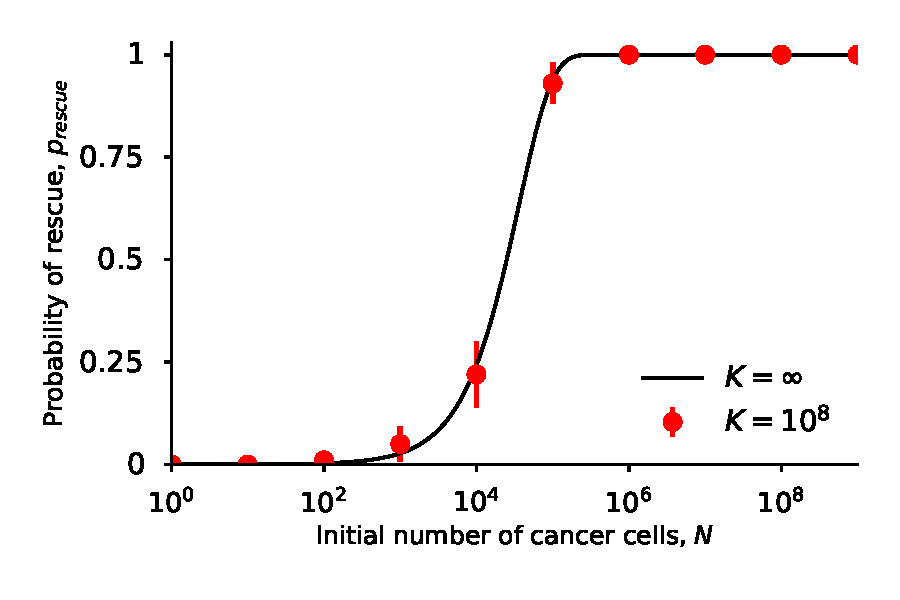
\includegraphics[width=1\textwidth]{Figures/SurvPlotNDataLogisticK.pdf}
\caption{\textbf{Density dependent growth does not affect the accuracy of our model.} Comparison of results of simulations  with density-dependent growth (red markers with with 95\% CI) and the approximation formula (black line, \cref{eq:N_a} in \cref{eq:rescue_prob}) with maximum carrying capacity $K=10^8$ and effective carrying capacity $K_e=K\Delta_a/\lambda_a\approx10^6$. The error bars represent $95\%$ confidence interval of the form $p\pm1.96\sqrt{p\left(1-p\right)/n}$ where $p$ is the  fraction of simulations in which the tumor has adapted to the stress and $n=100$ is the number of simulations. Parameters: $\lambda_s=0.1,\lambda_a=0.0901,\lambda_m=0.1,\mu_s=0.14,\mu_a=0.09,\mu_m=0.09, u=10^{-2}, v=10^{-7}, K=10^8$.}
\label{LogisticPlot}
\end{figure}
%%%
\begin{figure}[!htb]
\begin{subfigure}{0.5\textwidth}
A\\
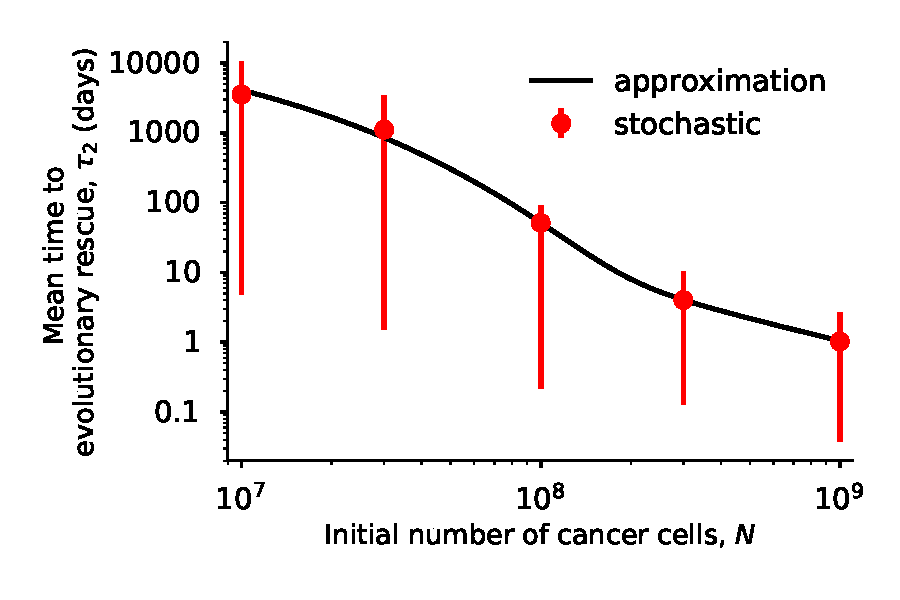
\includegraphics[width=1\textwidth]{Figures/EvolutionaryRescueTime.pdf}
\end{subfigure}
\begin{subfigure}{0.5\textwidth}
B\\
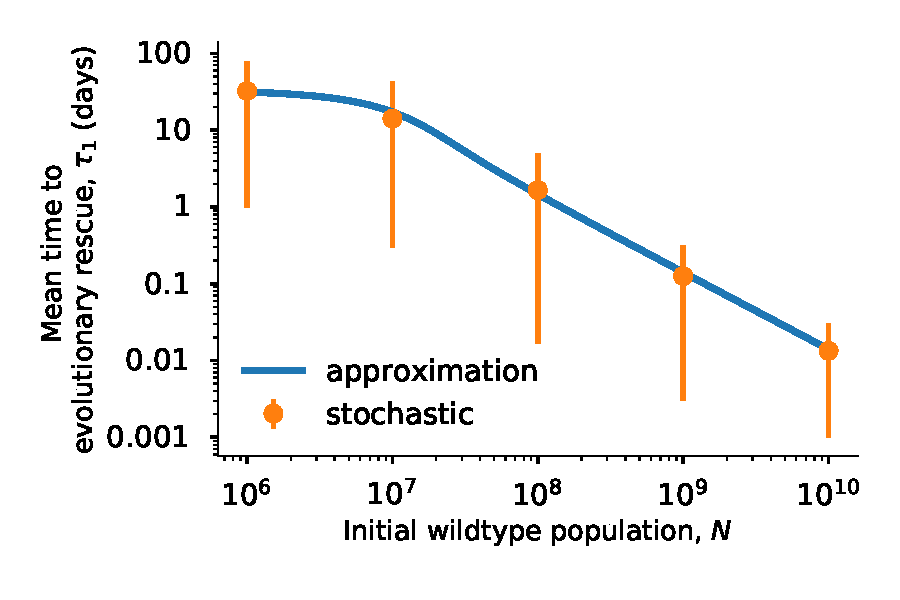
\includegraphics[width=1\textwidth]{Figures/MeanTimeGrowthMutantDirectPlot.pdf}
\end{subfigure}
\caption{\textbf{Evolutionary rescue time.}
Shown is the mean time for appearance of a resistance mutation that leads to evolutionary rescue (A) with aneuploidy ($u>0$) and (B) without aneuploidy ($u=0$).
Our inhomogeneous Poisson-process approximations (solid black lines, right: \cref{eq:meantime1}, left: \cref{meantimet2}) are in agreement with simulation results (red markers with 95\% quantile intervals obtained with bootstrapping, see see Appendix G). 
Parameters: $\lambda_s=0.1,\lambda_a=0.0899,\lambda_m=0.1,\mu_s=0.14,\mu_a=0.09,\mu_m=0.09, u=10^{-2}, v=10^{-7}$. %change 13
}
\label{MeanTimeGrowthAneuploidyPlot} 
\end{figure}
%%%
\begin{figure}
\vspace*{1\baselineskip}
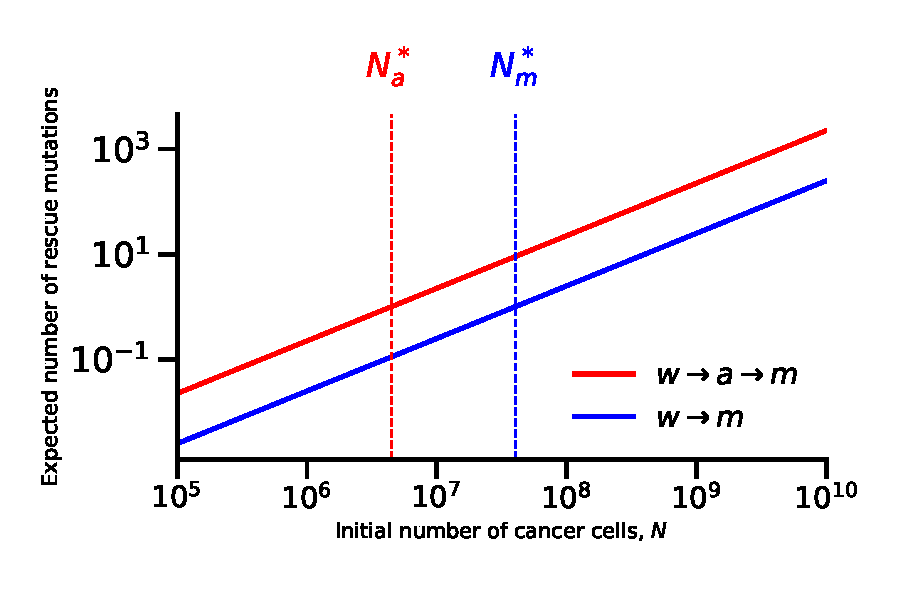
\includegraphics[width=1\textwidth]{Figures/ExpectedNumber.pdf}
\caption{\textbf{Aneuploidy increases the number of mutations which rescue the tumor.} Shown is the expected number of mutations, which will rescue the cancer cell population, produced through the evolutionary trajectory \textit{sensitive} $\rightarrow$ \textit{mutant} (blue line, \cref{eq:twosteplineagedirect}) or through the trajectory \textit{sensitive} $\rightarrow$ \textit{aneuploid} $\rightarrow$ \textit{mutant} (red line, \cref{eq:twosteplineage}). Dashed vertical red line represents the threshold tumor size above which evolutionary rescue is very likely through aneuploidy \cref{eq:N_a} and the dashed vertical blue line represents the threshold tumor size above which evolutionary rescue is very likely through direct mutation \cref{eq:N_m}.
Parameters: $\lambda_s=0.1,\lambda_a=0.0899,\lambda_m=0.1,\mu_s=0.14,\mu_a=0.09,\mu_m=0.09, u=10^{-2}, v=10^{-7}$.} %change 14
\label{ExpectedNumberRescueLineages}
\end{figure}
%%%
\begin{figure}
\vspace*{1\baselineskip}
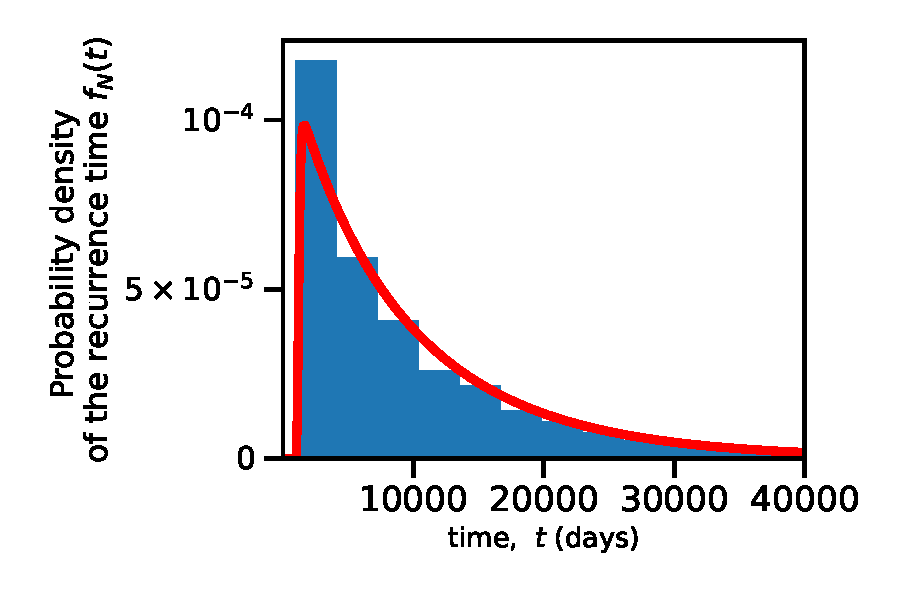
\includegraphics[width=1\textwidth]{Figures/KaplanMeierDistribution.pdf}
\caption{\textbf{Distribution of the recurrence time.}
Shown is the distribution of the time for the mutant cell population to reach size $N$, where $N$ is the initial number of cancer cells. The red line is analytic result \cref{distribution} overlaid over the histogram of simulations. 
Parameters: $N=10^6, \lambda_s=0.1,\lambda_a=0.0899,\lambda_m=0.1,\mu_s=0.14,\mu_a=0.09,\mu_m=0.09, u=10^{-2}, v=10^{-7}$.}
\label{KMdistribution}
\end{figure}
%%%
\begin{figure}
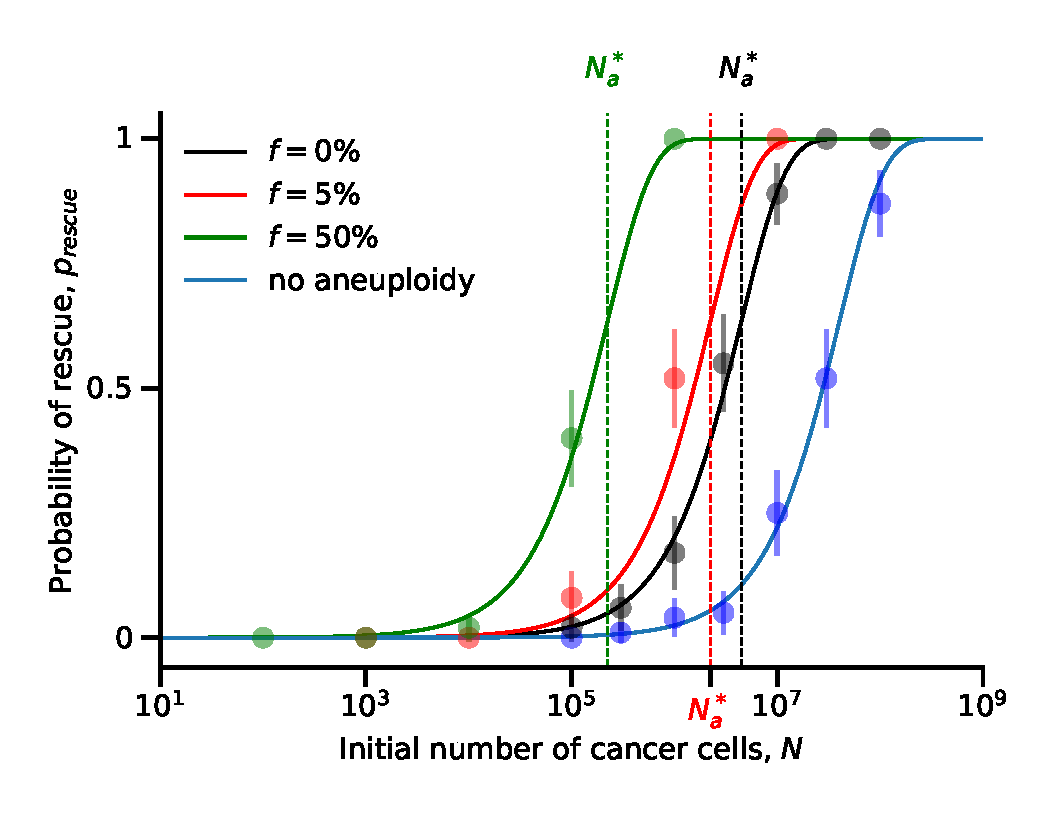
\includegraphics[width=1\textwidth]{Figures/ProbvN_SGV_Plot.pdf}
\caption{The probability of evolutionary rescue (i.e., the probability that the population does not go to extinction), $\presc$, as a function of the initial tumor size, $N$. Dashed vertical line shows the threshold tumor size, above which the probability is very high. Blue dashed line represents the probability of evolutionary rescue as a function of $N$ without aneuploidy ($u=0$). The black line represents the scenario where a fraction $f=0\%$ of the initial tumor is aneuploid, the red line represents the scenario with $f=5\%$ and the green line represents the scenario with $f=50\%$. The dots represent simulation results and the error bars represent $95\%$ confidence intervals ($p\pm1.96\sqrt{p\left(1-p\right)/n}$ where $p$ is the fraction of simulations in which the tumor has adapted to the stress and $n=100$ is the number of simulations). Parameters: $\lambda_s=0.1,\lambda_a=0.0899,\lambda_m=0.1,\mu_s=0.14,\mu_a=0.09,\mu_m=0.09, u=10^{-2}, v=10^{-7}$.} %change 15
\label{rescue_prob_sgv}
\end{figure}
%%%
\begin{figure}
\vspace*{1\baselineskip}
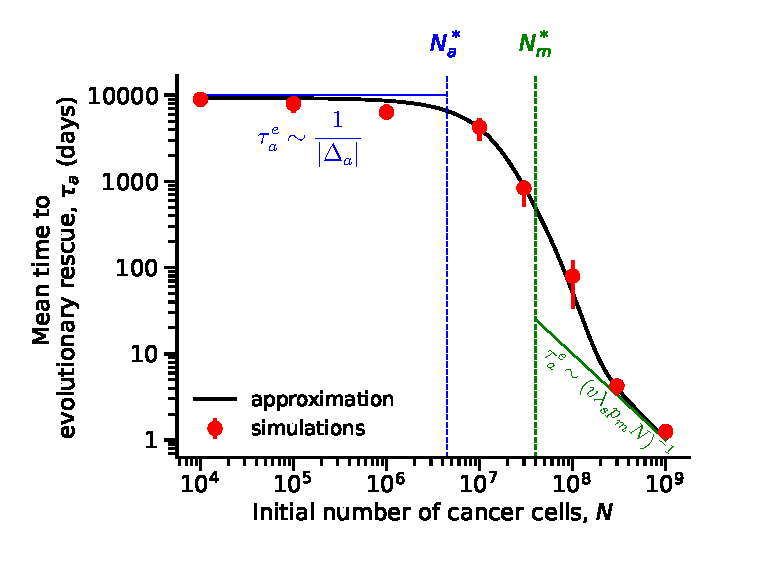
\includegraphics[width=1\textwidth]{Figures/EvolutionaryRescueTimeComplete.pdf} %change r5
\caption{The mean time for appearance of a resistance mutation that leads to evolutionary rescue with aneuploidy ($u>0$). 
Solid lines show our approximations (\cref{eq:AsymptoticTimeRules}) compared to red markers that show mean of simulations results (with error bars for 95\% confidence intervalues obtained with bootstrap, see Appendix G).
Blue dashed line, $N_a^*$.
Green dashed line, $N_m^*$.
Parameters: $\lambda_s=0.1,\lambda_m=0.0899,\lambda_a=0.1,\mu_s=0.14,\mu_a=0.09,\mu_m=0.09, u=10^{-2}, v=10^{-7}$.} %change 16
\label{EvolutionaryRescueTimeComplete}
\end{figure}
%%%
\begin{figure}
\vspace*{1\baselineskip}
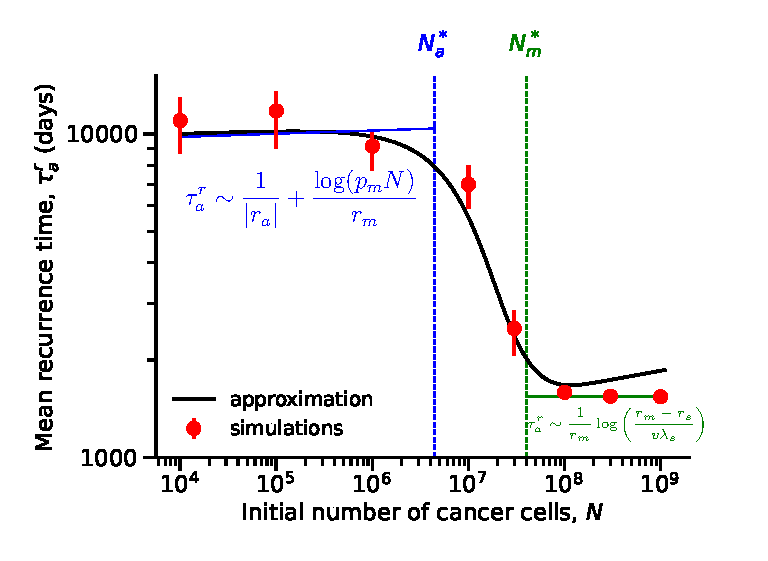
\includegraphics[width=1\textwidth]{Figures/ProliferationTimeLarge.pdf} %change r5
\caption{The mean time for the mutant cell population to reach size $N$, where $N$ is the initial number of cancer cells.
Solid lines show our approximations (green: \cref{eq:t2det}, blue: \cref{meanproliferationtime} with \cref{limitapprox4} for $\tau_a$; black: \cref{meanproliferationtime} with \cref{meantimet2} for $\tau_a$) compared to red markers that show mean of simulations results (with error bars for 95\% confidence intervals obtained with bootstrap, see Appendix G).
Blue dashed line, $N_a^*$.
Green dashed line, $N_m^*$.
Parameters: $\lambda_s=0.1,\lambda_a=0.0899,\lambda_m=0.1,\mu_s=0.14,\mu_a=0.09,\mu_m=0.09, u=10^{-2}, v=10^{-7}$.}
\label{ProliferationTimeLarge}
\end{figure}
%%%
\begin{figure}
\vspace*{1\baselineskip}
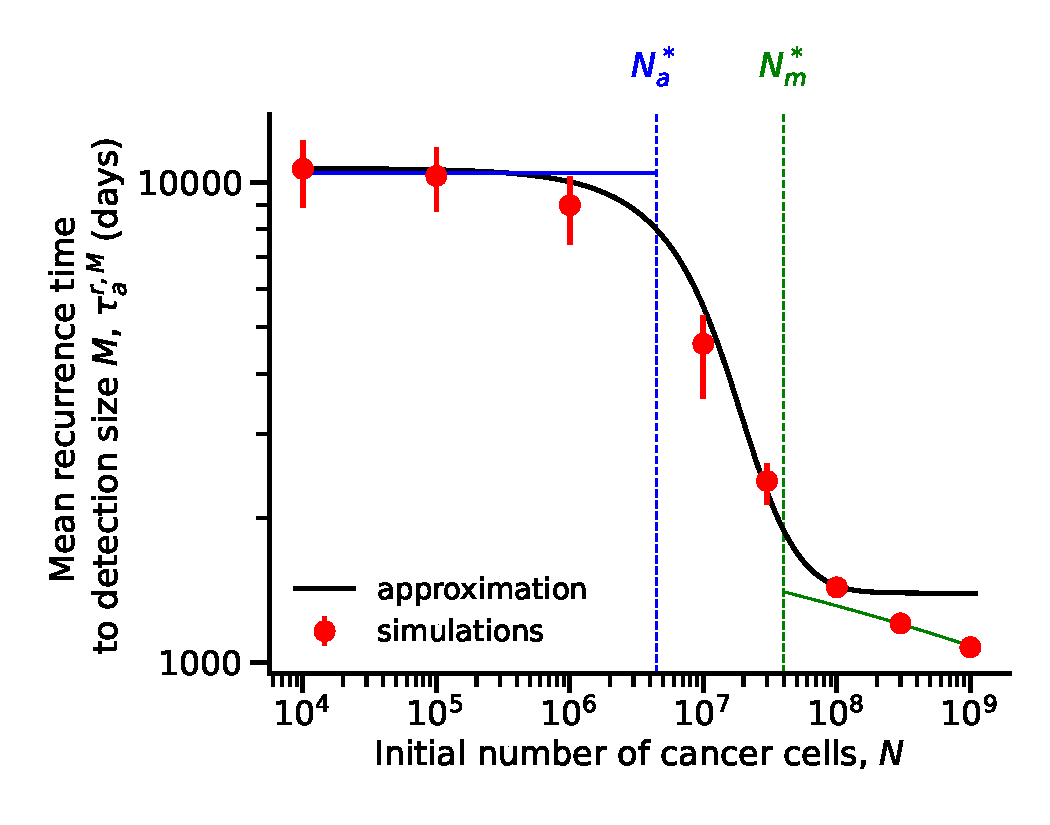
\includegraphics[width=1\textwidth]{Figures/RecurrencePlot.pdf} %change r5
\caption{The mean time for the mutant cell population to reach size $M$, where $M$ is the tumor detection size.
Solid lines show our approximations (green: \cref{eq:t2det2} for $N>N_m^*$, blue:  \cref{meanproliferationtime2} with $\tau_a$ from \cref{eq:AsymptoticTimeRules} for $N<N_a^*$; black: \cref{meanproliferationtime2}) compared to red markers that show mean of simulations results (with error bars for 95\% confidence intervals obtained with bootstrap, see Appendix G).
Blue dashed line, $N_a^*$.
Green dashed line, $N_m^*$.
Parameters: $\lambda_s=0.1,\lambda_a=0.0899,\lambda_m=0.1,\mu_s=0.14,\mu_a=0.09,\mu_m=0.09, u=10^{-2}, v=10^{-7}, M=10^7$.}
\label{RecurrencePlot}
\end{figure}
%%%
\begin{figure}
\vspace*{1\baselineskip}
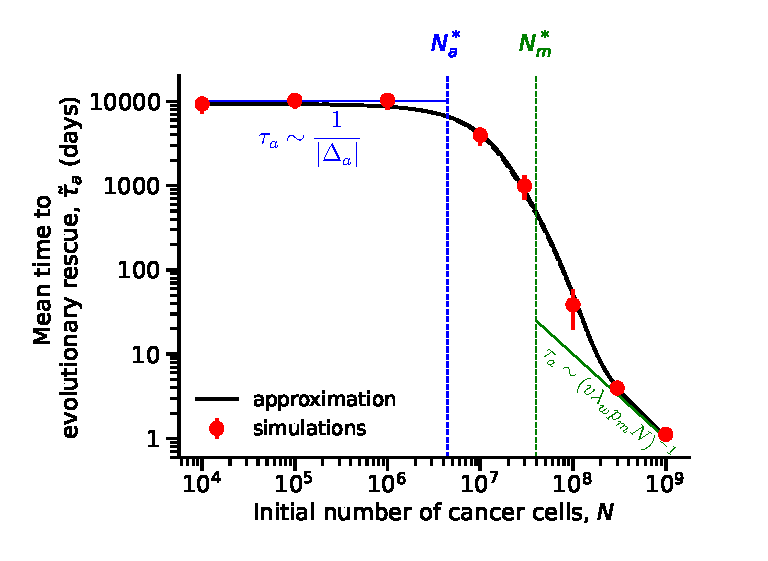
\includegraphics[width=1\textwidth]{Figures/SGVEvolutionaryRescueTimeComplete.pdf} %change r5
\caption{The mean time for appearance of a resistance mutation that leads to evolutionary rescue with aneuploidy ($u>0$) when a fraction $f$ of cancer cells are aneuploid at the start of drug treatment. 
Lines show our approximations (solid green: \cref{eq:AsymptoticTimeRules} for $N>N_m^*$; solid blue:  \cref{eq:AsymptoticTimeRules} for $N<N_a^*$; solid black: \cref{meantimet2}; dashed black: \cref{meantimet2SGV}) compared to red markers that show mean of simulations results (with error bars for 95\% confidence intervals obtained with bootstrap, see Appendix G).
Blue dashed line, $N_a^*$.
Green dashed line, $N_m^*$.
Parameters: $\lambda_s=0.1,\lambda_a=0.0899,\lambda_m=0.1,\mu_s=0.14,\mu_a=0.09,\mu_m=0.09, u=10^{-2}, v=10^{-7},f=0.14\%$.} %change 17
\label{SGVEvolutionaryRescueTimeComplete}
\end{figure}
%%%
\begin{figure}
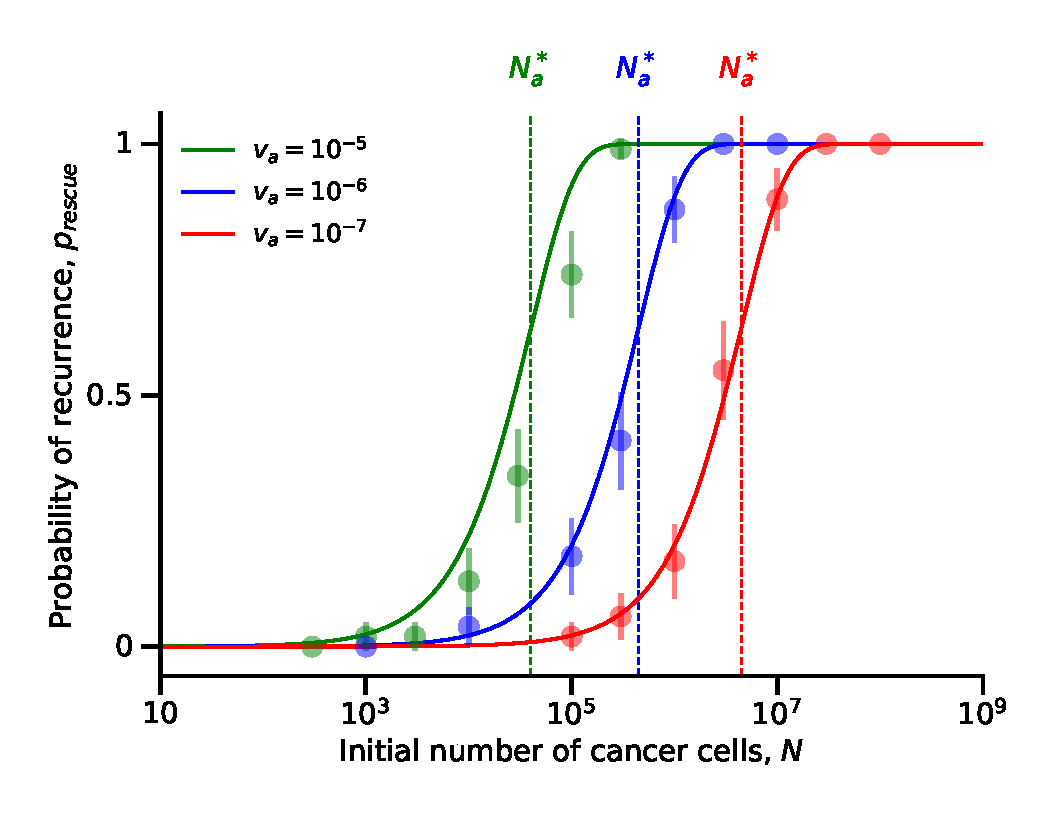
\includegraphics[width=1\textwidth]{Figures/ProbvNPlot_ane.pdf}
\caption{The probability of evolutionary rescue (i.e., the probability that the population does not become extinct), $\presc$, as a function of the initial tumor size, $N$ (\cref{eq:rescue_prob}). Dashed vertical line shows the threshold tumor size, $N_a^*$, above which the probability is very high (\cref{eq:N_a2}). Red dashed line: $v_a=10^{-7}$. blue line: $v_a=10^{-6}$. Green line: $v_a=10^{-5}$. Dots for simulations and the error bars for $95\%$ confidence interval ($p\pm1.96\sqrt{p\left(1-p\right)/n}$ where $p$ is the fraction of simulations in which the tumor has been rescued and $n=100$ is the number of simulations). Parameters: $\lambda_s=0.1,\lambda_m=0.1,\mu_s=0.14,\mu_a=0.09,\mu_m=0.09, u=10^{-2}, v_s=10^{-7}$.}
\label{rescue_prob_ane}
\end{figure}
\end{appendices}
%%%%%%%%%%%%%%%%%%%%%%%%%%%%%%%%%%%%%%%%%%
\end{document}